\documentclass[10pt]{beamer}
\usetheme[background=light,block=fill,progressbar=foot]{metropolis}


%% ctex configuration. slow compiling, comment unless using Chinese.
%\usepackage[UTF8]{ctex}
%\ctexset{refname=References}
%%

\usepackage{graphicx}
\usepackage{caption}
\usepackage{bm}
\usepackage{booktabs}
\usepackage{natbib}
\usepackage{algorithm}
\usepackage{algorithmic} 
\usepackage{transparent}
\newcommand{\supercite}[1]{\textsuperscript{\textsuperscript{\cite{#1}}}}
\newcommand{\emoji}[1]{\text{\raisebox{-0.2em}{\includegraphics[height=1em]{emojis/#1.png}}}}
\newcommand{\subtitlepage}[3]{\title{#1}\subtitle{#2}\author{#3}\date{}\begin{frame}[plain]\titlepage\end{frame}}
%\usefonttheme[onlymath]{serif}


\begin{document}
	\setbeamercovered{transparent=15}
	\setbeamertemplate{caption}{\raggedright\insertcaption\par}
	
	\title{A Brief Review on GANs}
	\subtitle{From Computer Vision to Natural Language Processing}
	\author{Bothan Shi \\ botianshi@bit.edu.cn}
	\date{Apr, 13, 2017}
	
	
	\begin{frame}[plain]
		\titlepage
	\end{frame}

	\part{Outline}
	\begin{frame}{Outline}
		\begin{figure}
			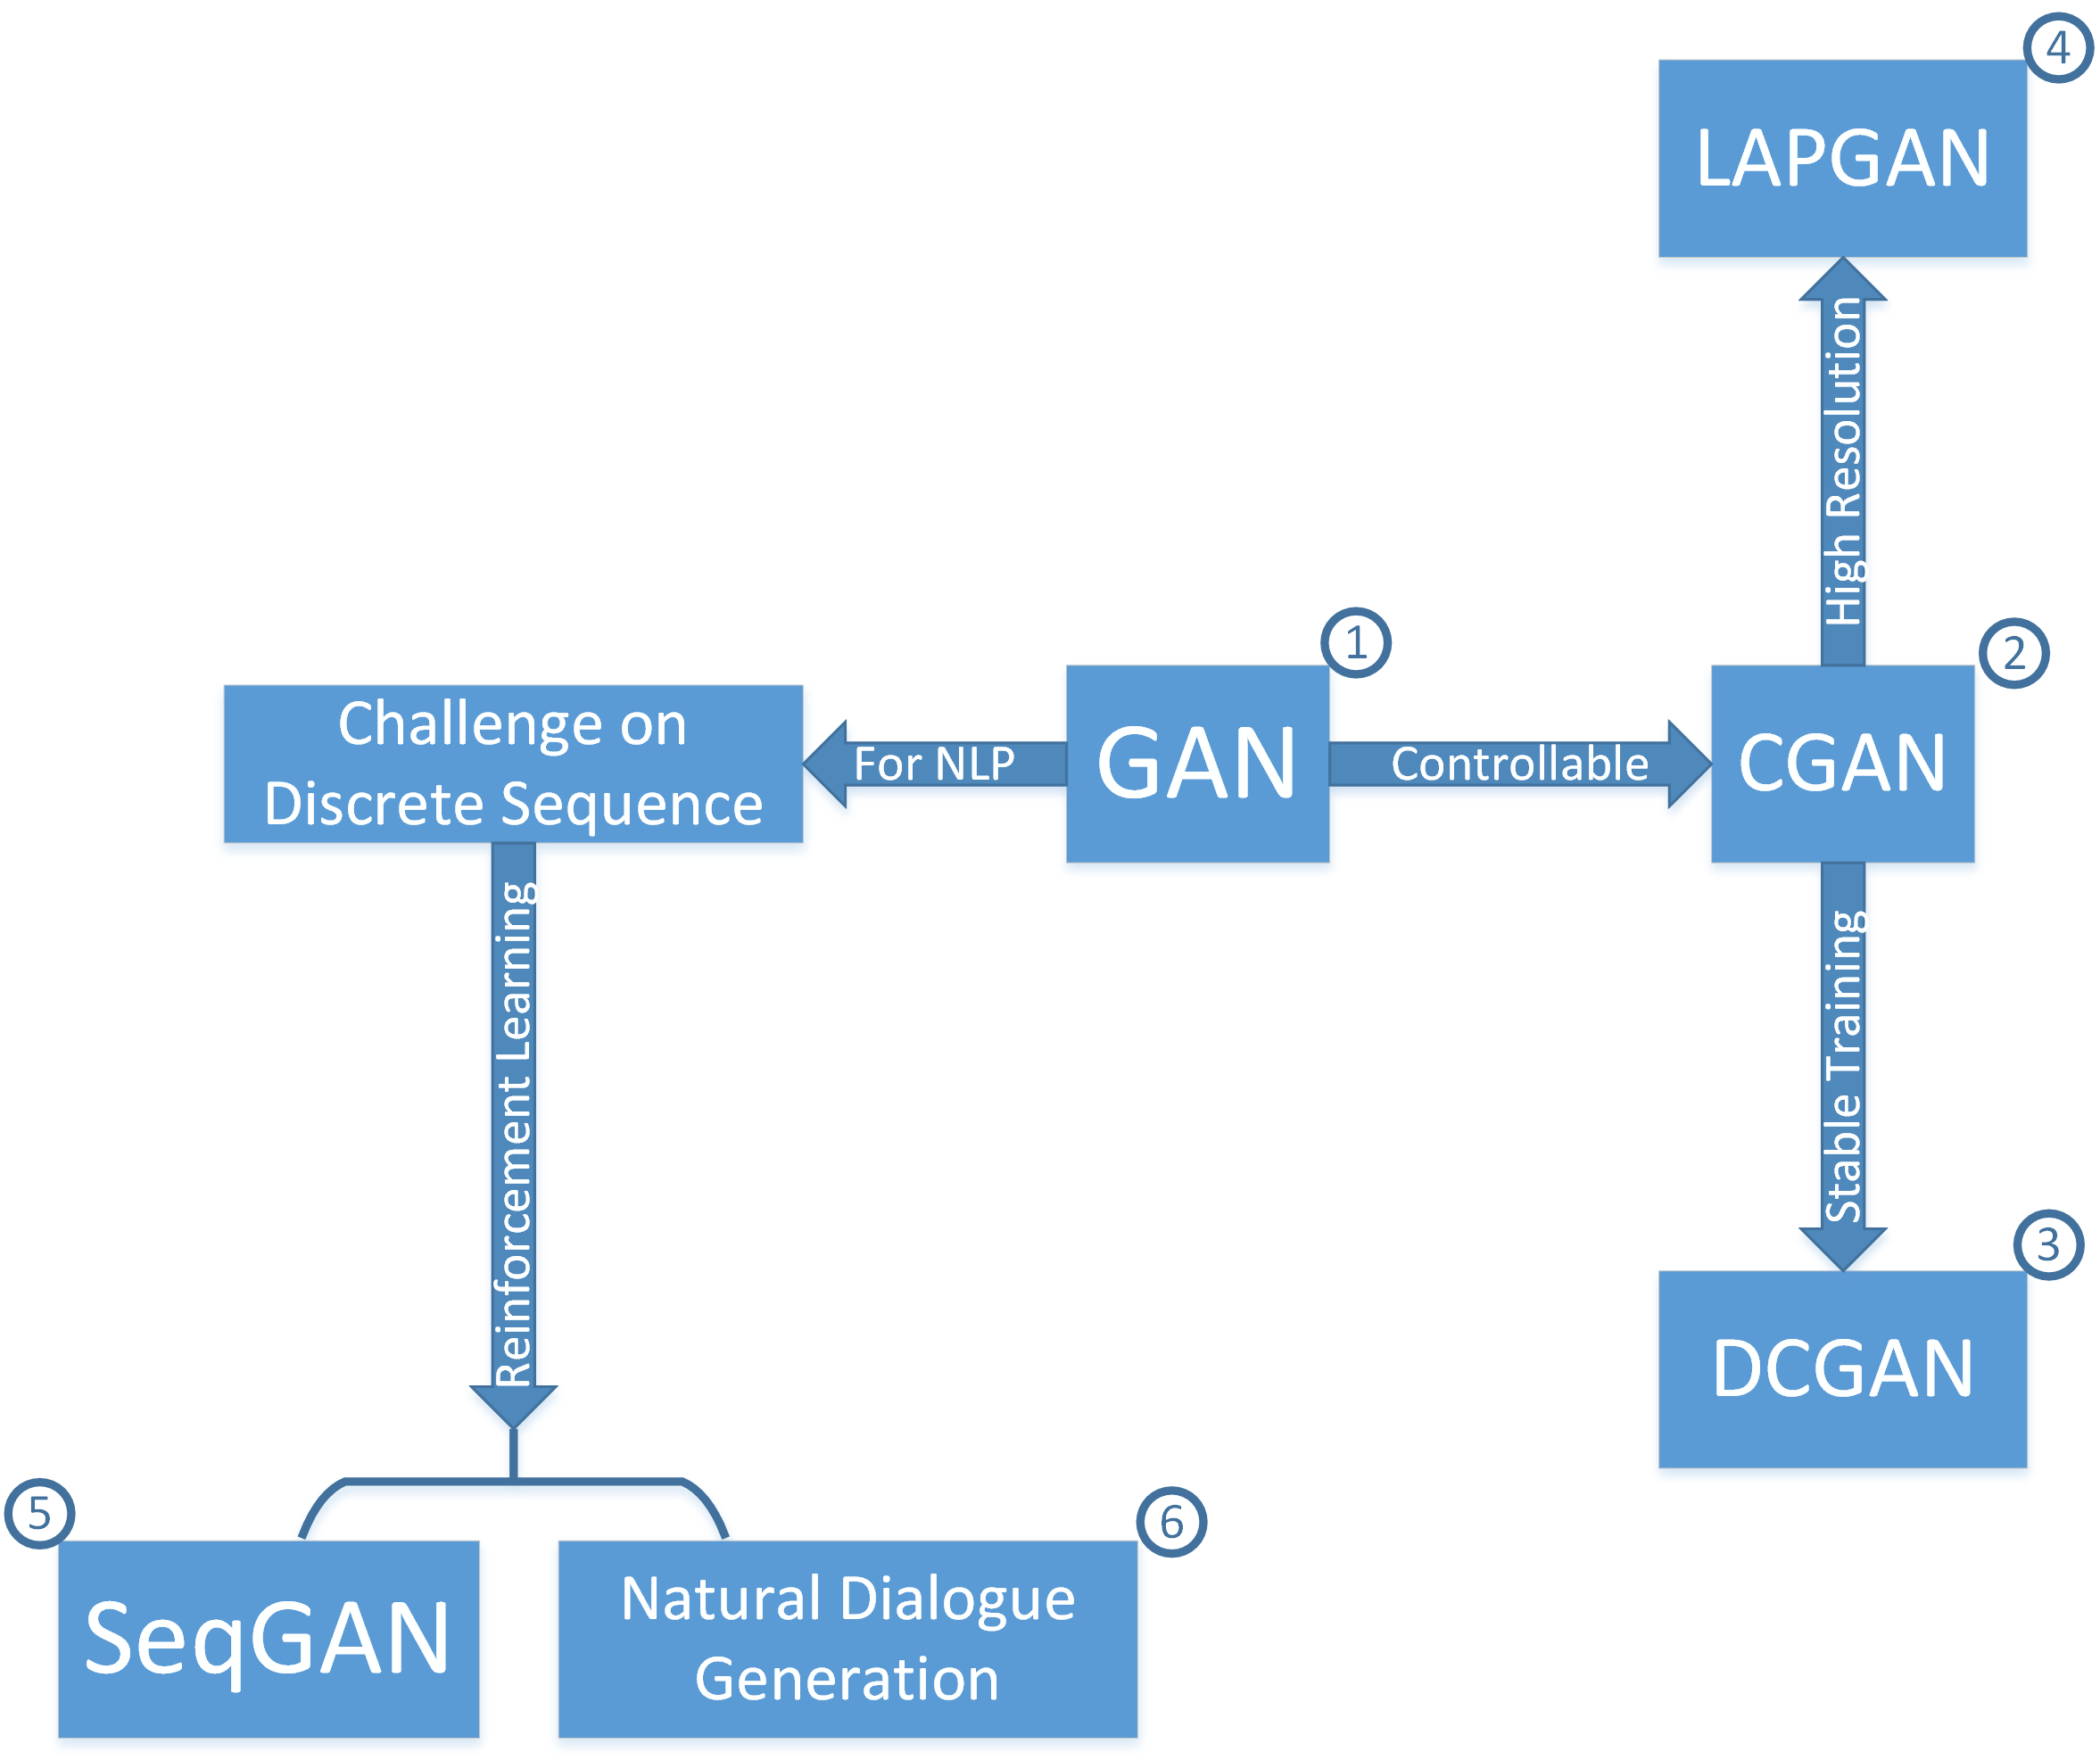
\includegraphics[width=25em]{figures/outline.png}
		\end{figure}
	\end{frame}

	\part{Background: Generative Model and Discriminative Model}
	\subtitlepage{Background Information}{Generative Model and Discriminative Model}{}
	\begin{frame}{Generative Model and Discriminative Model}
		What is generative model?
		\begin{itemize}
			\pause
			\item Modelling the generation distribution of data.
			\pause
			\item Done by modelling a joint probability distribution $p(x, y)$.
		\end{itemize}
		\pause
		What is discriminative model?
		\begin{itemize}
			\pause
			\item Modelling the dependence of an unobserved variable $y$ on an observed variable $x$.
			\pause
			\item Done by modelling the conditional probability distribution $p(y|x)$.
			\pause
			\item For tasks such as classification and regression that do not require the joint distribution, discriminative models can yield superior performance.
		\end{itemize}
		\pause
		\textbf{generative models modelling the data, discriminative models modelling the difference between data}.
	\end{frame}

	\begin{frame}{Generative Model and Discriminative Model}
		Why we need generative model?
		\begin{itemize}
			\pause
			\item We can get a discriminative model via a generative model by $p(y|x)=\frac{p(x, y)}{p(x)}$, the other way not. 
			\pause
			\item We can \textbf{sample new data} from generative model whereas discriminative model cannot. (AMAZING!)
		\end{itemize}
		\pause
		Is is easy to get a generative model?
		\begin{itemize}
			\pause
			\item It is hard to estimate an probabilistic model.
			\pause
			\item We need enough observed data + robust model.
		\end{itemize}
		\pause
		How can we get a generative model?
		\begin{itemize}
			\pause
			\item Gaussian mixture model and other types (GMM)
			\pause
			\item Hidden Markov Model (HMM)
			\pause
			\item Latent Dirichlet Allocation(LDA)
			\pause
			\item Restricted Boltzmann Machine (RBM)
			\pause
			\item \textbf{Generative Adversarial Networks (GAN)}
		\end{itemize}
	\end{frame}

	\part{GAN}
	\subtitlepage{}{Generative Adversarial Nets}{Ian J. Goodfellow, Jean Pouget-Abadie, Mehdi Mirza, Bing Xu, \\ David Warde-Farley, Sherjil Ozair, Aaron Courville, Yoshua Bengio. \\ NIPS 2014\\ arXiv: 1406.2661}
	
	\begin{frame}{Introduction of GAN}
		\begin{itemize}
			\pause
			\item New framework for estimating generative models via an adversarial process.
			\pause
			\item Train two models simultaneously:
			\begin{itemize}
				\pause
				\item A generative model $G$ that captures the data distribution.
				\pause
				\item A discriminative model $D$ that estimates the probability that a sample came from the training data rather than $G$.
			\end{itemize}
			\pause
			\item A minimax two-player zero-sum game.
			\pause
			\item Unique solution exists (ensuring convergence): $G$ recovering the training data distribution; $D=\frac{1}{2}$ everywhere.
		\end{itemize}
	\end{frame}

	\begin{frame}{Introduction of GAN}
		\begin{itemize}
			\item The purpose of generative model is to learn data distribution $p_g$.
			\pause
			\item We have a noise variable $p_z(z)$ first, and sample a $z\sim p_z(z)$.
			\pause
			\item Synthesized data $\hat{x}=G(z;\theta_g)$. $\theta_g$ is the parameter of the generative model.
			\pause
			\item If the $\theta_g$ is well trained, we will get a generative model $p_g\approx p_{\text{data}}$. ($p_g$ have learned the same mapping function as $p_{\text{data}}$)
			\pause
			\item In this case, we can generate new "fake" data realistic enough to confuse human as well as the discriminator.
			\pause
			\item AMAZING! Our model has learned the distribution of data and can generate new sample! For example: produce "reasonable" images.
		\end{itemize}
	\end{frame}

	\begin{frame}{Adversarial nets}
		\begin{figure}
			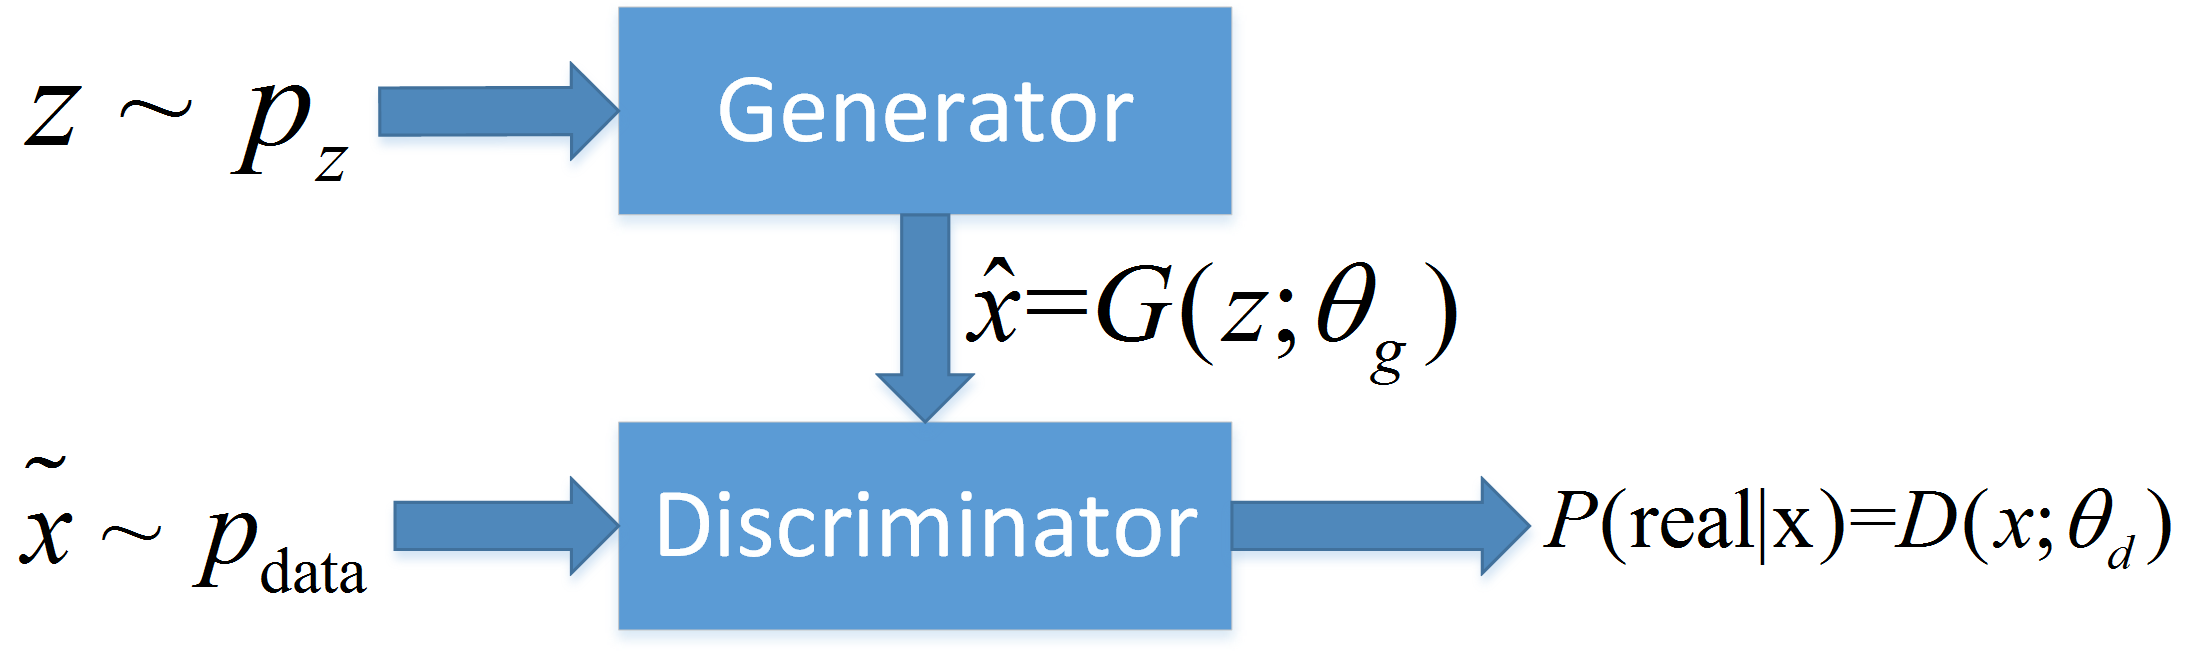
\includegraphics[width=25em]{figures/GAN-general-structure.png}
		\end{figure}
		\pause
		We train $D$ to maximize the probability of assigning the correct label to both training examples and samples from $G$.
		
		\pause
		We simultaneously train $G$ to minimize $\log(1-D(G(\bm{z})))$. In other words, $D$ and $G$ play the following two-player minimax game with value function $V(G,D)$:
		\pause
		$$
		\mathop{\min}_{G}\mathop{\max}_{D}V(D,G)=\mathbb{E}_{\bm{x}\sim p_{\text{data}}}\left[\log D(\bm{x})\right]+\mathbb{E}_{\bm{z}\sim p_z(\bm{z})}\left[\log(1-D(G(\bm{z})))\right].
		$$
		
	\end{frame}

	\begin{frame}{Adversarial nets}
		\onslide<1->
		Why we need the discriminator? Why can't we define the loss function as the MSE of the real image and the image produced by the generator directly?
		\onslide<2->
		\begin{figure}
			\only<1>{\mbox{\phantom{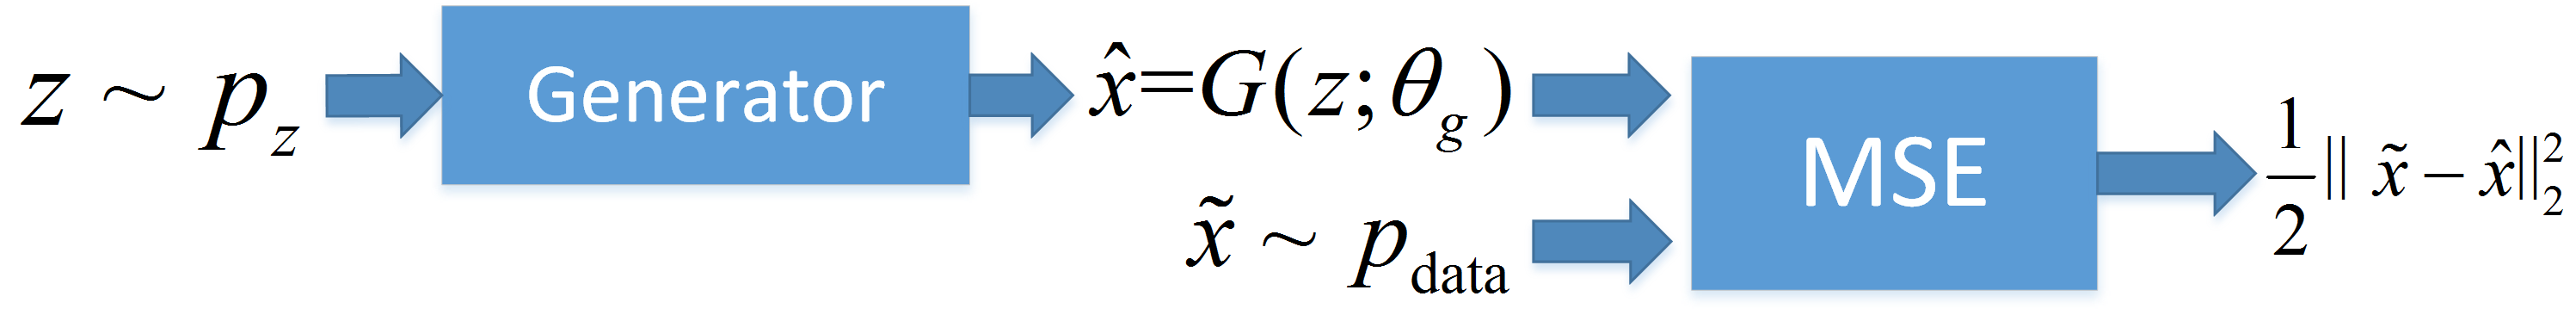
\includegraphics[width=25em]{figures/GAN-hypothesis-structure.png}}}}
			\includegraphics<2->[width=25em]{figures/GAN-hypothesis-structure.png}
		\end{figure}
		\onslide<3->
		If we only have the generator, this model can be regarded as an unsupervised learning problem. 
		
		\onslide<4->
		But if we want the output image of the generator as similar as possible to the training sample, the generator will finally remember all the training data and it will not be able to produce any "new" images.
	\end{frame}

	\begin{frame}[t]{Adversarial nets}
		\onslide<1->
		Here is a less formal, more pedagogical explanation of the approach:
		\onslide<2->
		\begin{figure}
			\only<1>{\mbox{\phantom{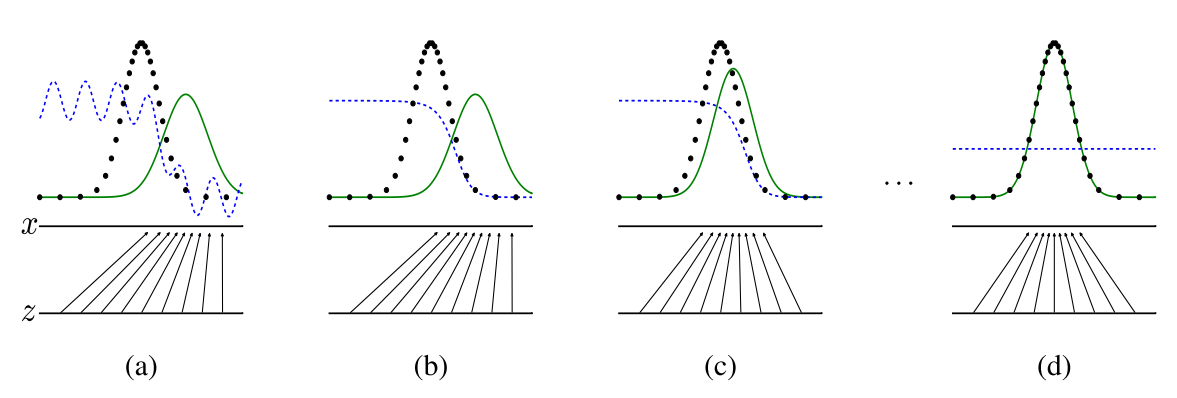
\includegraphics[width=25em]{figures/GAN-pedagogical-explanation.png}}}}
			\includegraphics<2->[width=25em]{figures/GAN-pedagogical-explanation.png}
		\end{figure}
		\onslide<3->
		Generative adversarial nets are trained by simultaneously updating the \textbf{d}iscriminative distribution (D, blue, dashed line) so that it discriminates between samples from the data generating distribution (black, dotted line) $p_g$ from those of the \textbf{g}enerative distribution $p_g(G)$ (green, solid line). 
	\end{frame}
	
	\begin{frame}[t]{Adversarial nets}
		Here is a less formal, more pedagogical explanation of the approach:
		\begin{figure}
			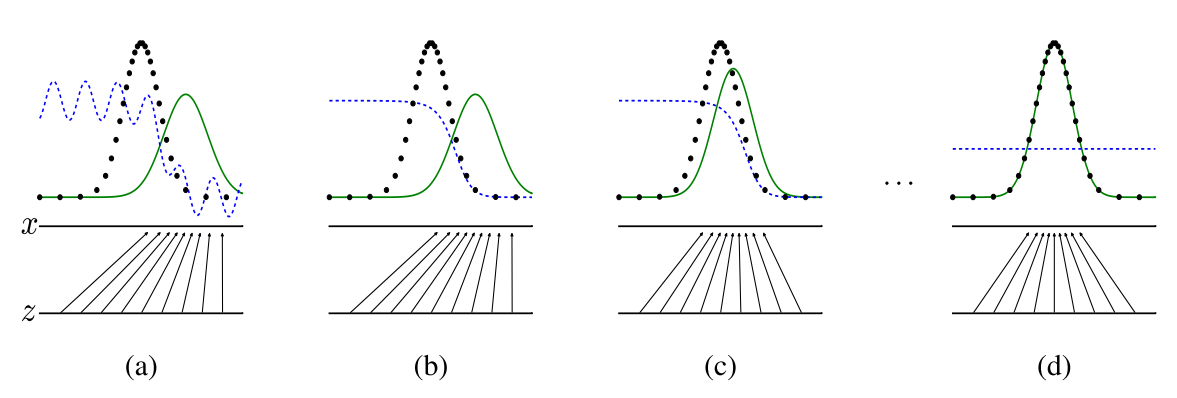
\includegraphics[width=25em]{figures/GAN-pedagogical-explanation.png}
		\end{figure}
	 	The lower horizontal line is the domain from which $\bm{z}$ is sampled, in this case uniformly. The horizontal line above is part of the domain of $\bm{x}$. The upward arrows show how the mapping $\bm{x}=G(\bm{z})$ imposes the non-uniform distribution $p_g$ on transformed samples.
	\end{frame}

	\begin{frame}[t]{Adversarial nets}
		Here is a less formal, more pedagogical explanation of the approach:
		\begin{figure}
			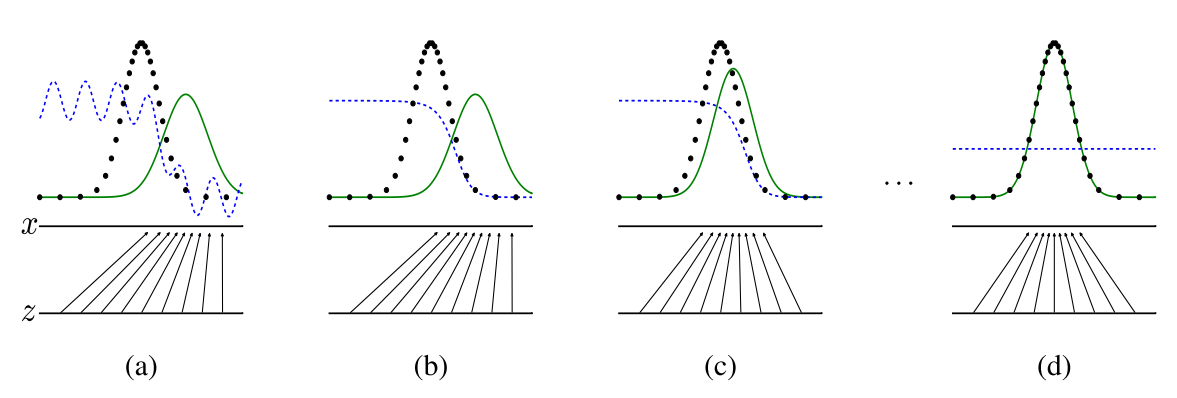
\includegraphics[width=25em]{figures/GAN-pedagogical-explanation.png}
		\end{figure}
		(a) Consider an adversarial pair near convergence: $p_g$ is similar to $p_{\text{data}}$ and $D$ is a partially accurate classifier.
		
		\pause
		(b) In the inner loop of the algorithm $D$ is trained to discriminate samples from data, converging to $D^*(\bm{x})=\frac{p_{\text{data}}(\bm{x})}{p_{\text{data}}(\bm{x})+p_g(\bm{x})}$
	\end{frame}

	\begin{frame}[t]{Adversarial nets}
		Here is a less formal, more pedagogical explanation of the approach:
		\begin{figure}
			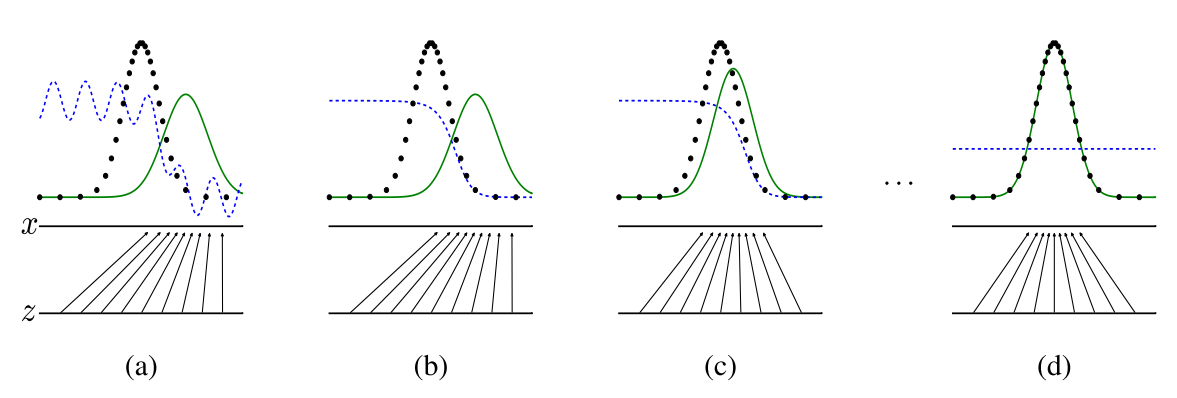
\includegraphics[width=25em]{figures/GAN-pedagogical-explanation.png}
		\end{figure}
		(c) After an update to $G$, gradient of $D$ has guided $G(\bm{z})$ to flow to regions that are more likely to be classified as data.
		
		\pause
		(d) After several steps of training, if $G$ and $D$ have enough capacity, they will reach a point at which both cannot improve because $p_g=p_{\text{data}}$.
	\end{frame}

	\begin{frame}[t]{Adversarial nets}
		Here is a less formal, more pedagogical explanation of the approach:
		\begin{figure}
			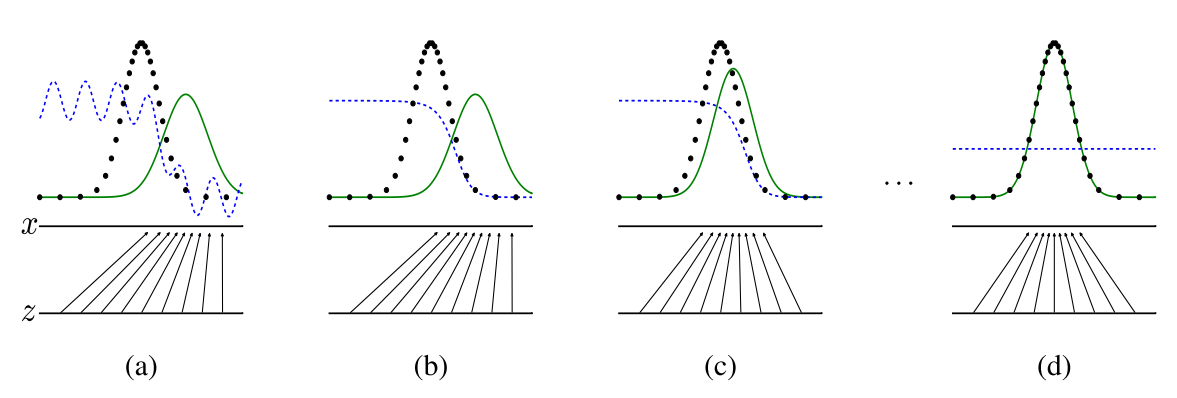
\includegraphics[width=25em]{figures/GAN-pedagogical-explanation.png}
		\end{figure}
		The discriminator is unable to differentiate between the two distributions. i.g. $D(\bm{x})=\frac{1}{2}$
	\end{frame}

	\begin{frame}{Adversarial nets}
		\begin{itemize}
			\item There are several trifles we need to deal with. The first is insufficient gradient in the early learning.
			\pause
			\item Let's take a look at the loss function again:
			\pause
			$$
			\mathop{\min}_{G}\mathop{\max}_{D}V(D,G)=\mathbb{E}_{\bm{x}\sim p_{\text{data}}}\left[\log D(\bm{x})\right]+\mathbb{E}_{\bm{z}\sim p_z(\bm{z})}\left[\log(1-D(G(\bm{z})))\right].
			$$
			\pause
			\item In practice, this equation may not provide sufficient gradient for $G$ to learn well.
			\pause
			\item Early in learning, when $G$ is poor, $D$ can reject samples with high confidence because they are clearly different from the training data.
			\pause
			\item In this case, $\log(1-D(G(z)))$ saturates.
			\pause
			\item Rather than training $G$ to minimize $\log(1-D(G(\bm{z})))$ we can train $G$ to maximize $\log D(G(\bm{z}))$.
			\pause
			\begin{eqnarray*}
			&&\mathop{\max}_{D}\mathbb{E}_{\bm{x}\sim p_{\text{data}}}\left[\log D(\bm{x})\right]+\mathbb{E}_{\bm{z}\sim p_z(\bm{z})}\left[\log(1-D(G(\bm{z})))\right] \\
			&&\mathop{\max}_{G}\mathbb{E}_{\bm{z}\sim p_{\text{z}}}\left[\log D(G(\bm{z}))\right]
			\end{eqnarray*}
		\end{itemize}
	\end{frame}

	\begin{frame}{Adversarial nets}
		\begin{itemize}
			\item The second trifle is that we need to prevent the overfit of $G$.
			\pause
			\item We should conduct the iterative training: optimize the discriminator $k$ times and then train the generator once. 
			\pause
		\end{itemize}
		\begin{algorithm}[H]
			\algsetup{linenosize=\tiny}
			\scriptsize
			%\tiny
			%\captionsetup{labelformat=empty}
			\caption*{\textbf{Algorithm} \scriptsize Minibatch stochastic gradient descent training of generative adversarial nets.}
			\label{alg:train-gan}
			\begin{algorithmic}
				\pause
				\FOR{number of training iterations}
					\pause
					\FOR{$k$ steps}
						\pause
						\STATE Sample minibatch of $m$ noise samples $\{z^{(1)},\dots,z^{(m)}\}$ from noise prior $p_g(\bm{z})$
						\pause
						\STATE Sample minibatch of $m$ examples ${x^{(1)},\dots,x^{(m)}}$ from data generating distribution $p_{\text{data}}(\bm{x})$
						\pause
						\STATE Update the discriminator by ascending its stochastic gradient:
							\pause
							\vspace{-1em}
							$$
							\nabla_{\theta_{d}}\frac{1}{m}\sum^m_{i=1}\left[\log D\left(\bm{x}^{(i)}\right)+\log\left(1-D\left(G\left(\bm{z}^{(i)}\right)\right)\right)\right]
							$$
							\vspace{-1em}
					\ENDFOR
					\pause
					\STATE Sample minibatch of $m$ noise samples ${z^{(1)},\dots,z^{(m)}}$ from noise prior $p_g(\bm{z})$.
					\pause
					\STATE Update the generator by descending its stochastic gradient:
						\pause
						\vspace{-1em}
						$$
						\nabla_{\theta_{g}}\frac{1}{m}\sum_{i=1}^{m}\log\left(1-D\left(G\left(\bm{z}^{(i)}\right)\right)\right)
						$$
						\vspace{-1em}
				\ENDFOR
			\end{algorithmic}
		\end{algorithm}
	\end{frame}

	\begin{frame}{Experiments}
		\begin{itemize}
			\item MNIST.
			\item Toronto Face Database(TFD).
			\item CIFAR-10.
		\end{itemize}
		\begin{figure}
			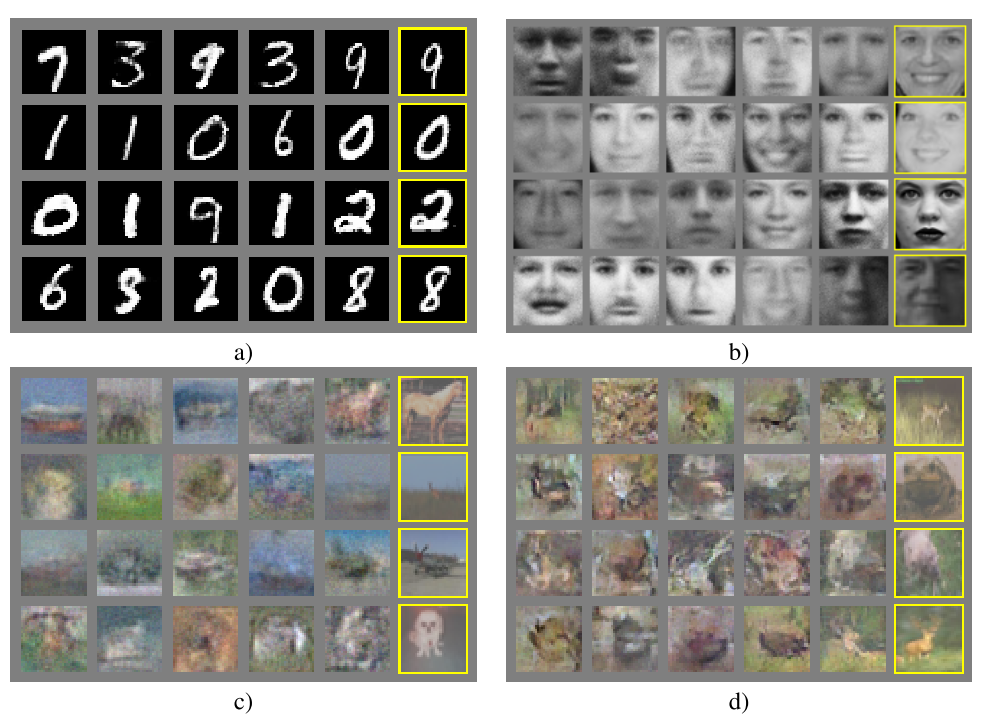
\includegraphics[width=25em]{figures/GAN-experiment-demo-pic.png}
		\end{figure}
	\end{frame}

	\part{CGAN}
	\begin{frame}{Outline}
		\begin{figure}
			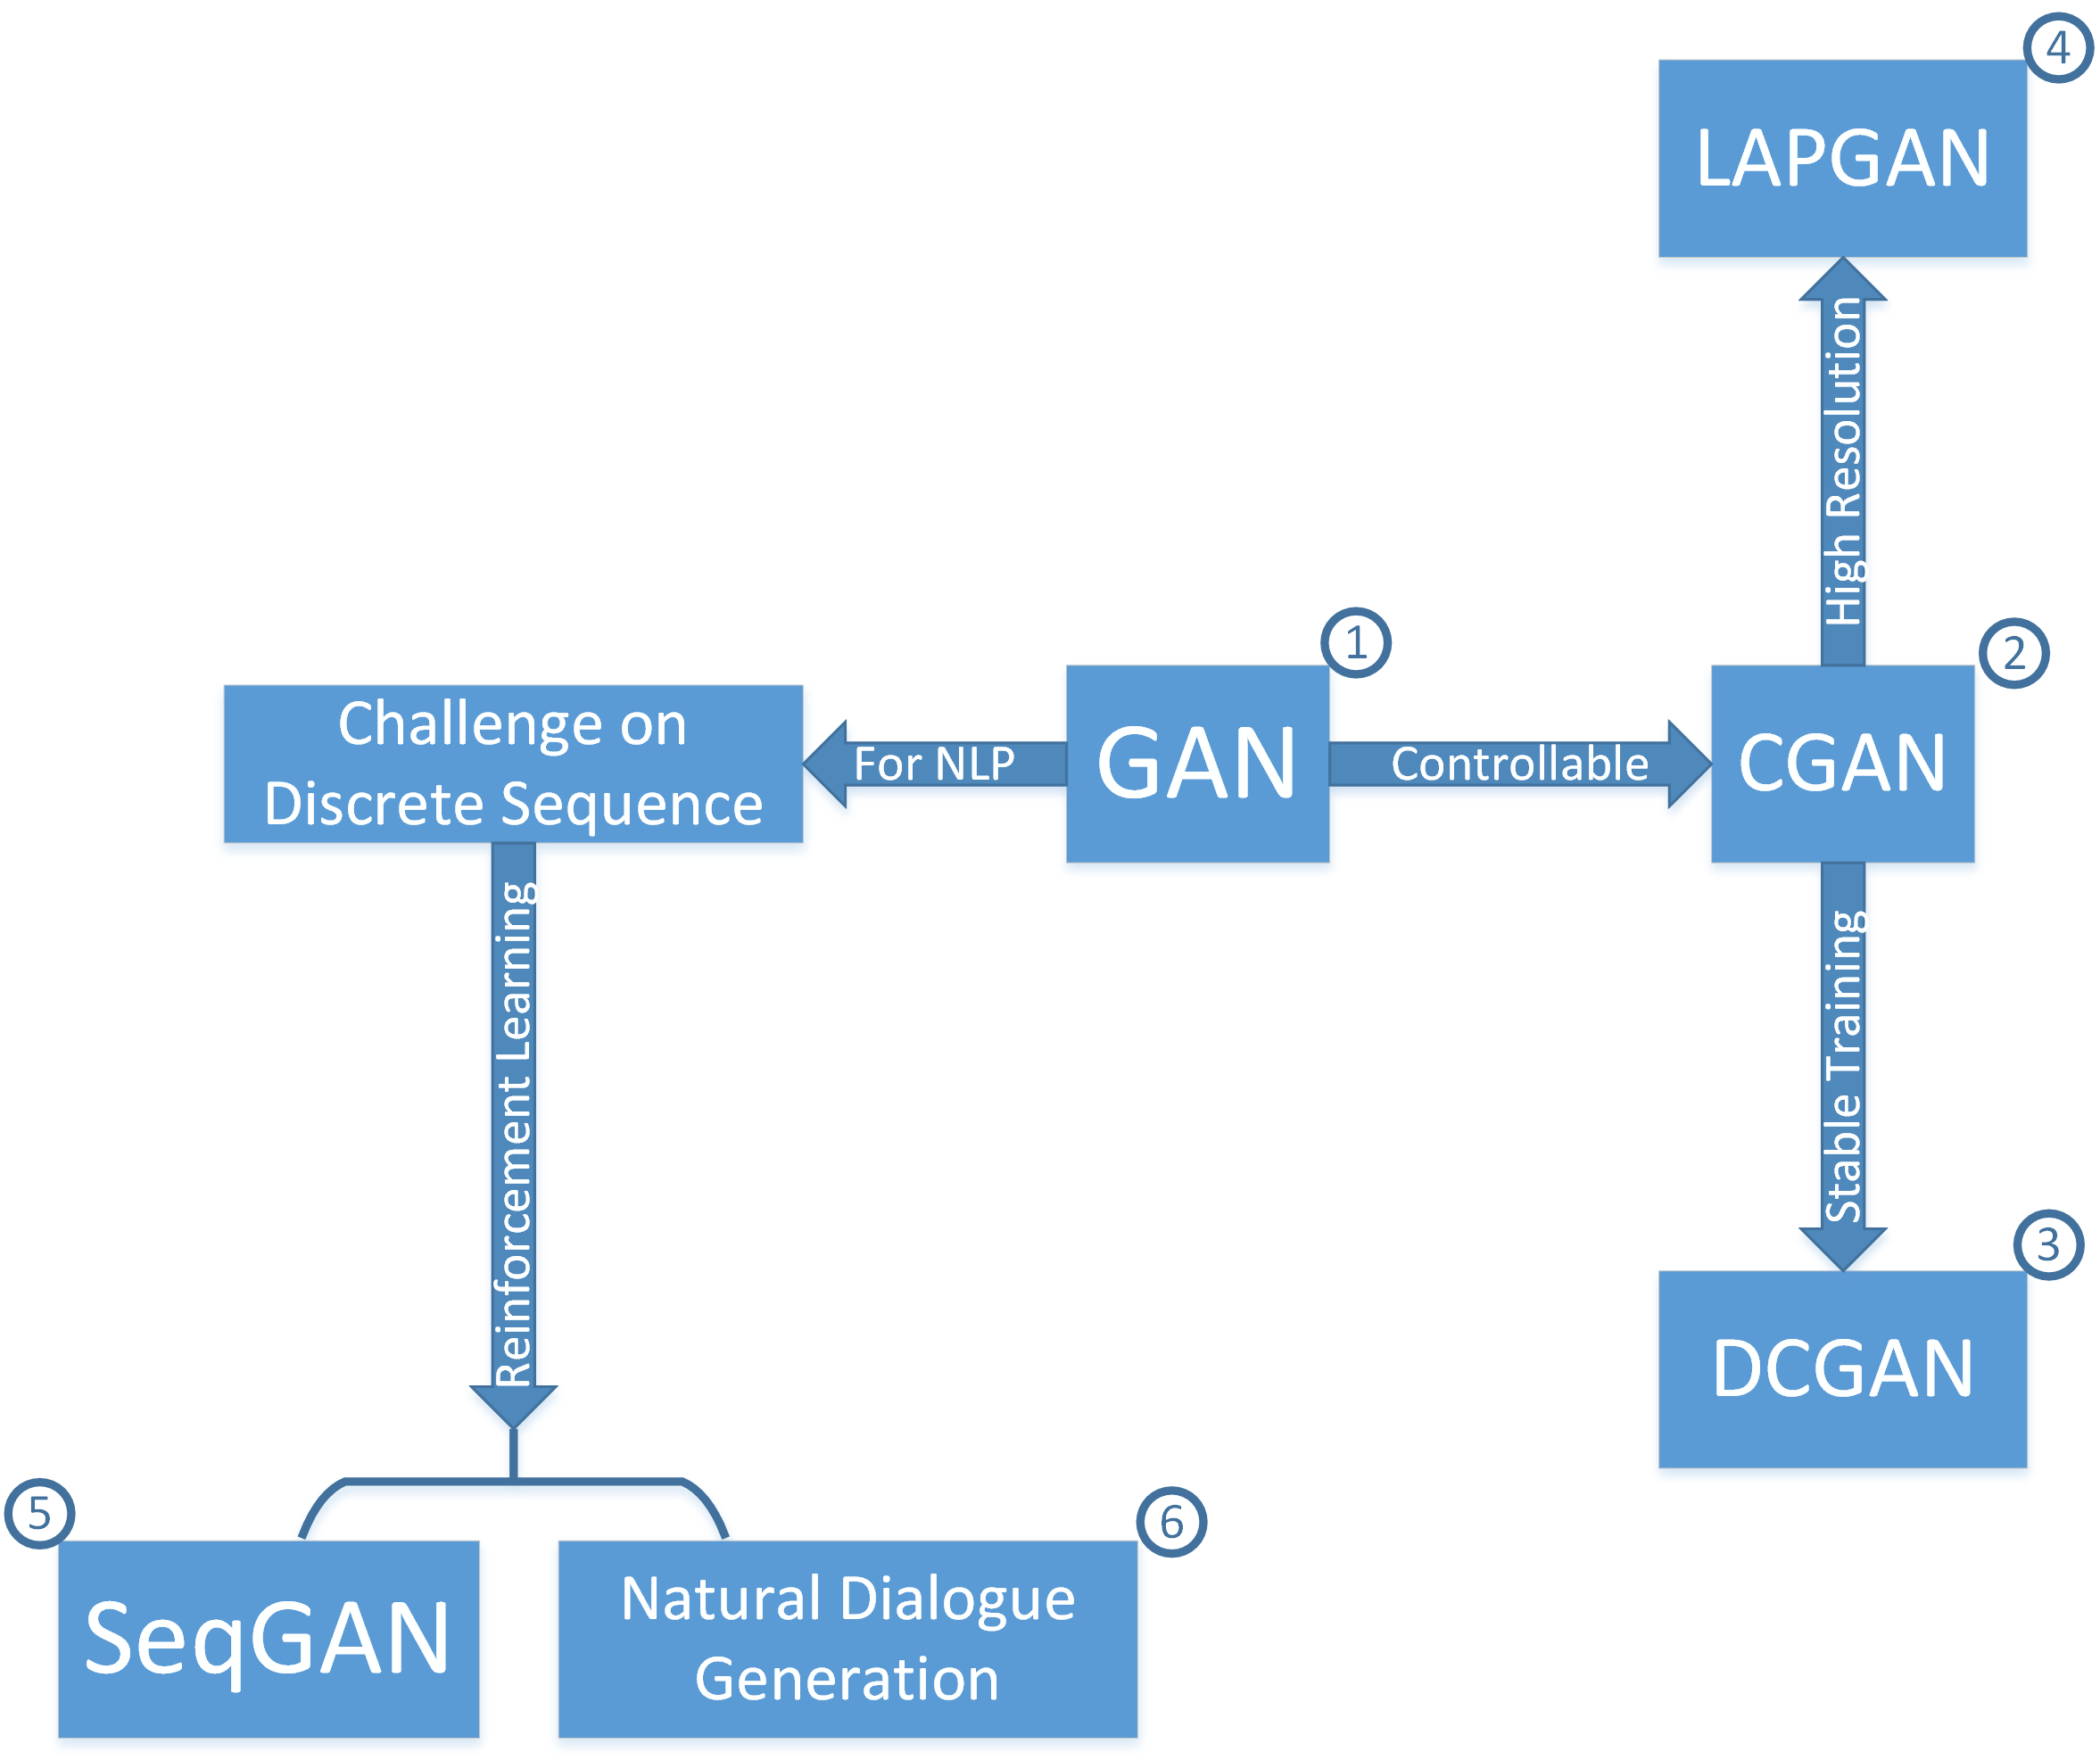
\includegraphics[width=25em]{figures/outline.png}
		\end{figure}
	\end{frame}
	\subtitlepage{}{Conditional Generative Adversarial Nets}{Mehdi Mirza, Simon Osindero\\arXiv: 1411.1784}
	
	\begin{frame}{Introduction}
		\begin{itemize}
			\item Generative adversarial nets were recently introduced as an alternative framework for training generative models.
			\pause
			\item In an unconditioned generative model, there is no control on models of the data being generated.
			\pause
			\item By conditioning the model on additional information it is possible to direct the data generating process.
			\pause
			\item Such conditioning could be based on class labels, on some part of data, or even on data from different modality.
		\end{itemize}
	\end{frame}

	\begin{frame}{CGAN and GAN}
		\begin{itemize}
			\pause
			\item Optimization object of unconditioned generative model:
			\pause
			$$
			\mathop{\min}_{G}\mathop{\max}_{D}V(D,G)=\mathbb{E}_{\bm{x}\sim p_{\text{data}}}\left[\log D(\bm{x})\right]+\mathbb{E}_{\bm{z}\sim p_z(\bm{z})}\left[\log(1-D(G(\bm{z})))\right].
			$$
			\pause
			\item Optimization object of conditioned generative model:
			\pause
			$$
			\mathop{\min}_{G}\mathop{\max}_{D}V(D,G)=\mathbb{E}_{\bm{x}\sim p_{\text{data}}}\left[\log D(\bm{x}|\bm{y})\right]+\mathbb{E}_{\bm{z}\sim p_z(\bm{z})}\left[\log(1-D(G(\bm{z}|\bm{y})|\bm{y}))\right].
			$$
		\end{itemize}
	\end{frame}

	\begin{frame}{Structure}
		\begin{figure}
			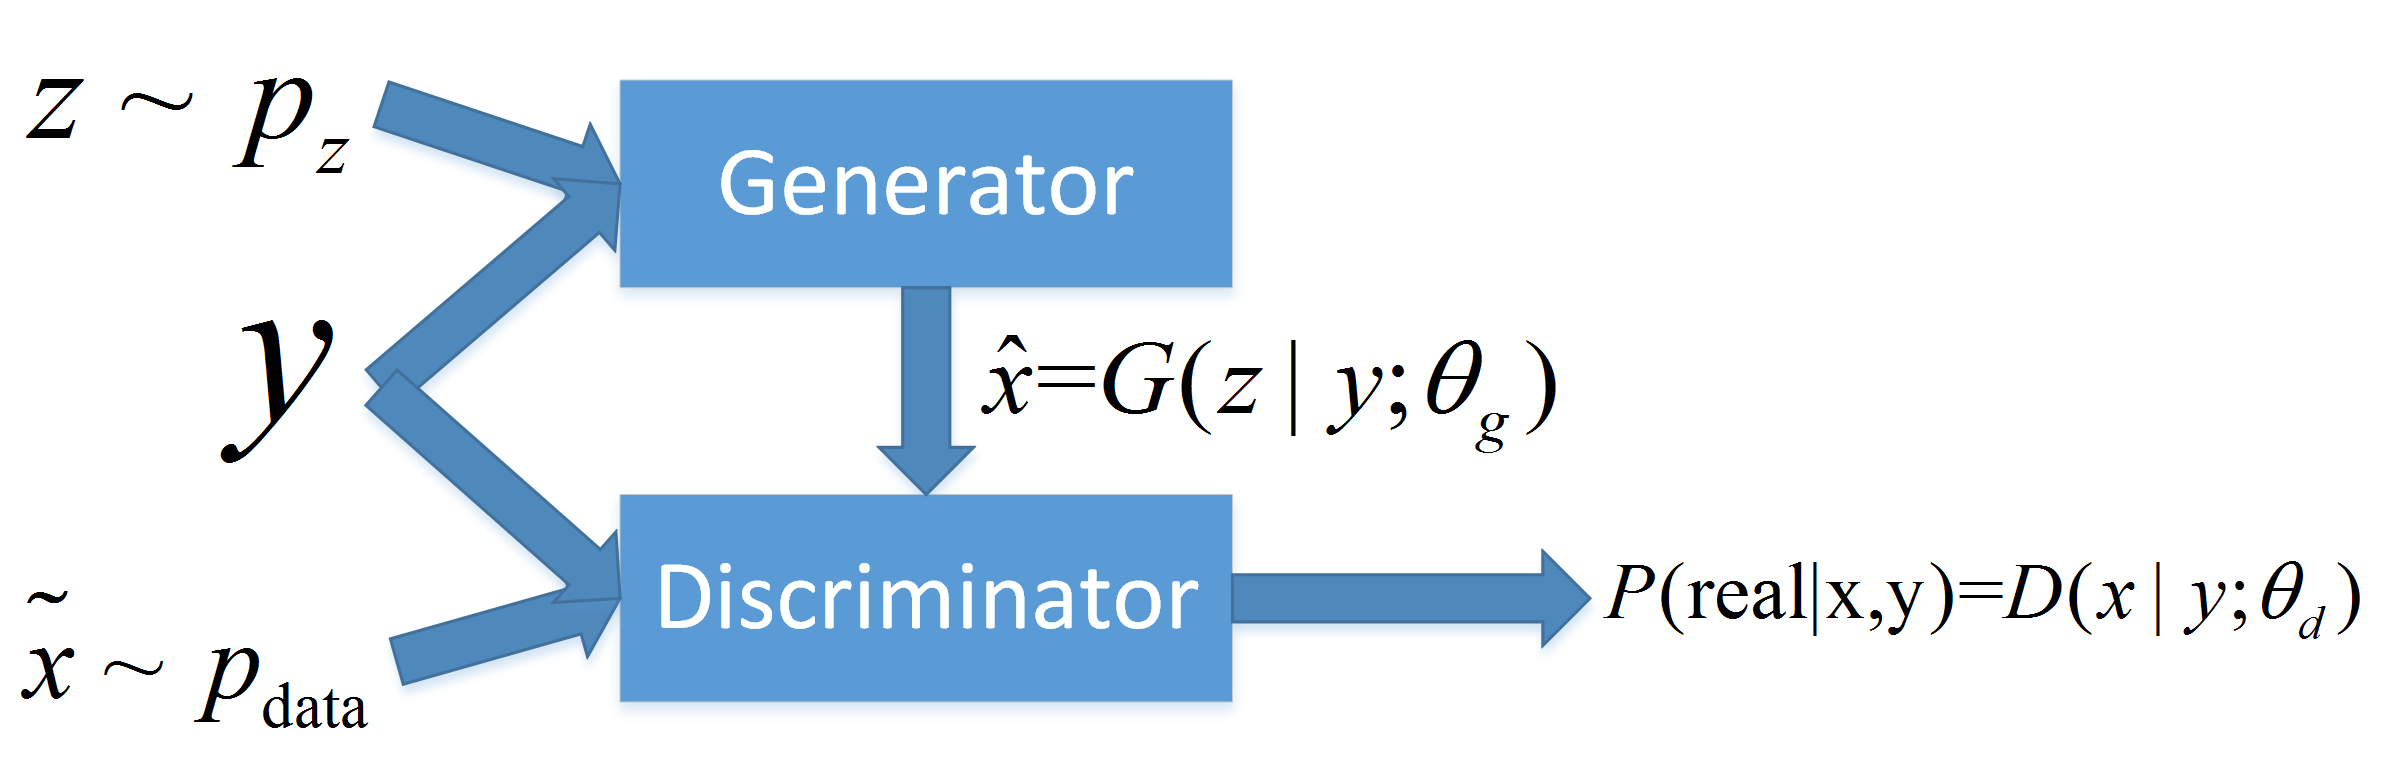
\includegraphics[width=20em]{figures/CGAN-general-structure.png}
		\end{figure}
		\begin{figure}
			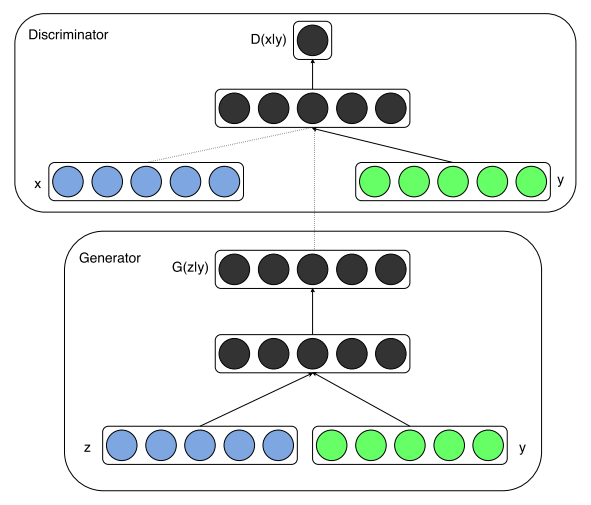
\includegraphics[width=15em]{figures/CGAN-origin-structure.png}
		\end{figure}
	\end{frame}

	\begin{frame}{Experiment}
		\begin{itemize}
			\onslide<1->
			\item Experiment on MNIST.
			\onslide<2->
			\item $y$ is the 10 classes of digit represent in one-hot vector.
			\onslide<3->
			\begin{figure}
				\only<1-2>{\mbox{\phantom{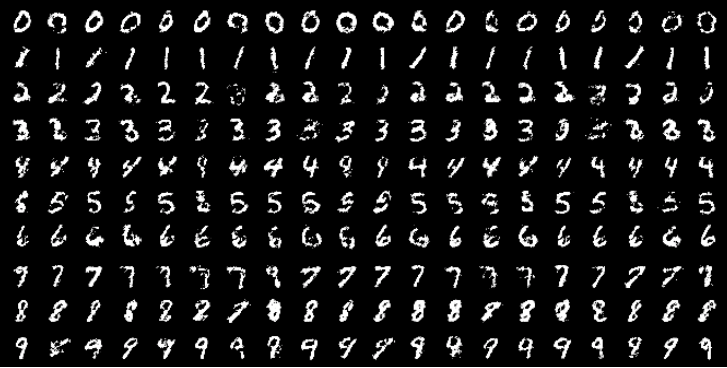
\includegraphics[width=25em]{figures/CGAN-experiment-mnist.png}}}}
				\includegraphics<3->[width=25em]{figures/CGAN-experiment-mnist.png}
				\caption{Generated MNIST digits, each row conditioned on one label}
			\end{figure}
		\end{itemize}
	\end{frame}

	\begin{frame}{Experiment (Multi-modal)}
		\begin{itemize}
			\pause
			\item Pretrained image feature extractor and skip-gram model for word representation.
			\pause
			\item Trained a convolutional image feature extractor on full ImageNet dataset.
			\pause
			\item Trained a skip-gram model for word representation: a $\mathrm{R}^{200}$ word vector on YFCC100M(Yahoo Flickr Creative Common 100M) dataset meta-data.
			\pause
			\item Conducted experiment on MIR Flickr 25,000 dataset, extract the image and tags features using the convolution model and embedding model.
		\end{itemize}
	\end{frame}

	\begin{frame}{Experiment (Multi-modal)}
		\begin{figure}
			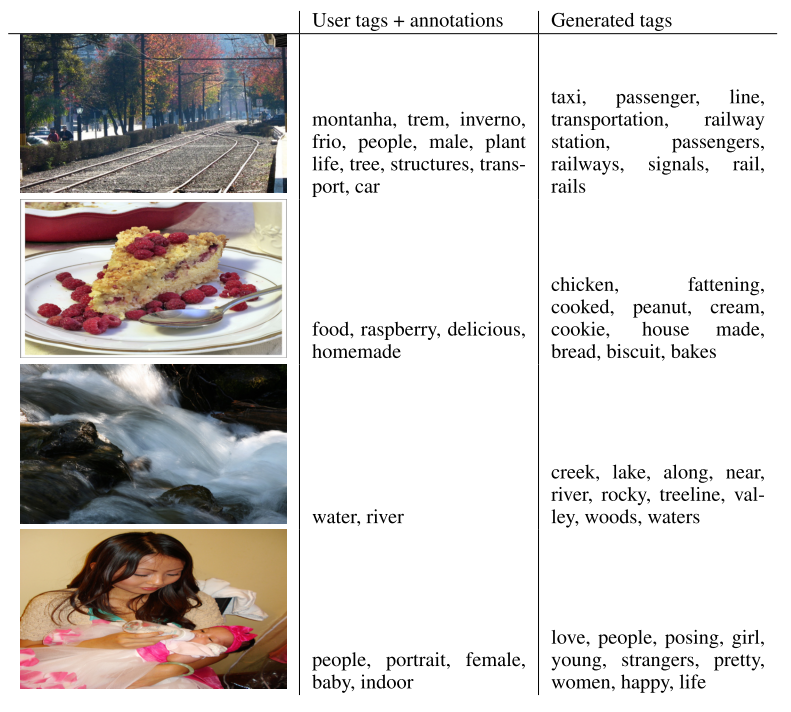
\includegraphics[width=25em]{figures/CGAN-experiment-multi-modal.png}
		\end{figure}
	\end{frame}
	
	\part{DCGAN}
	\begin{frame}{Outline}
		\begin{figure}
			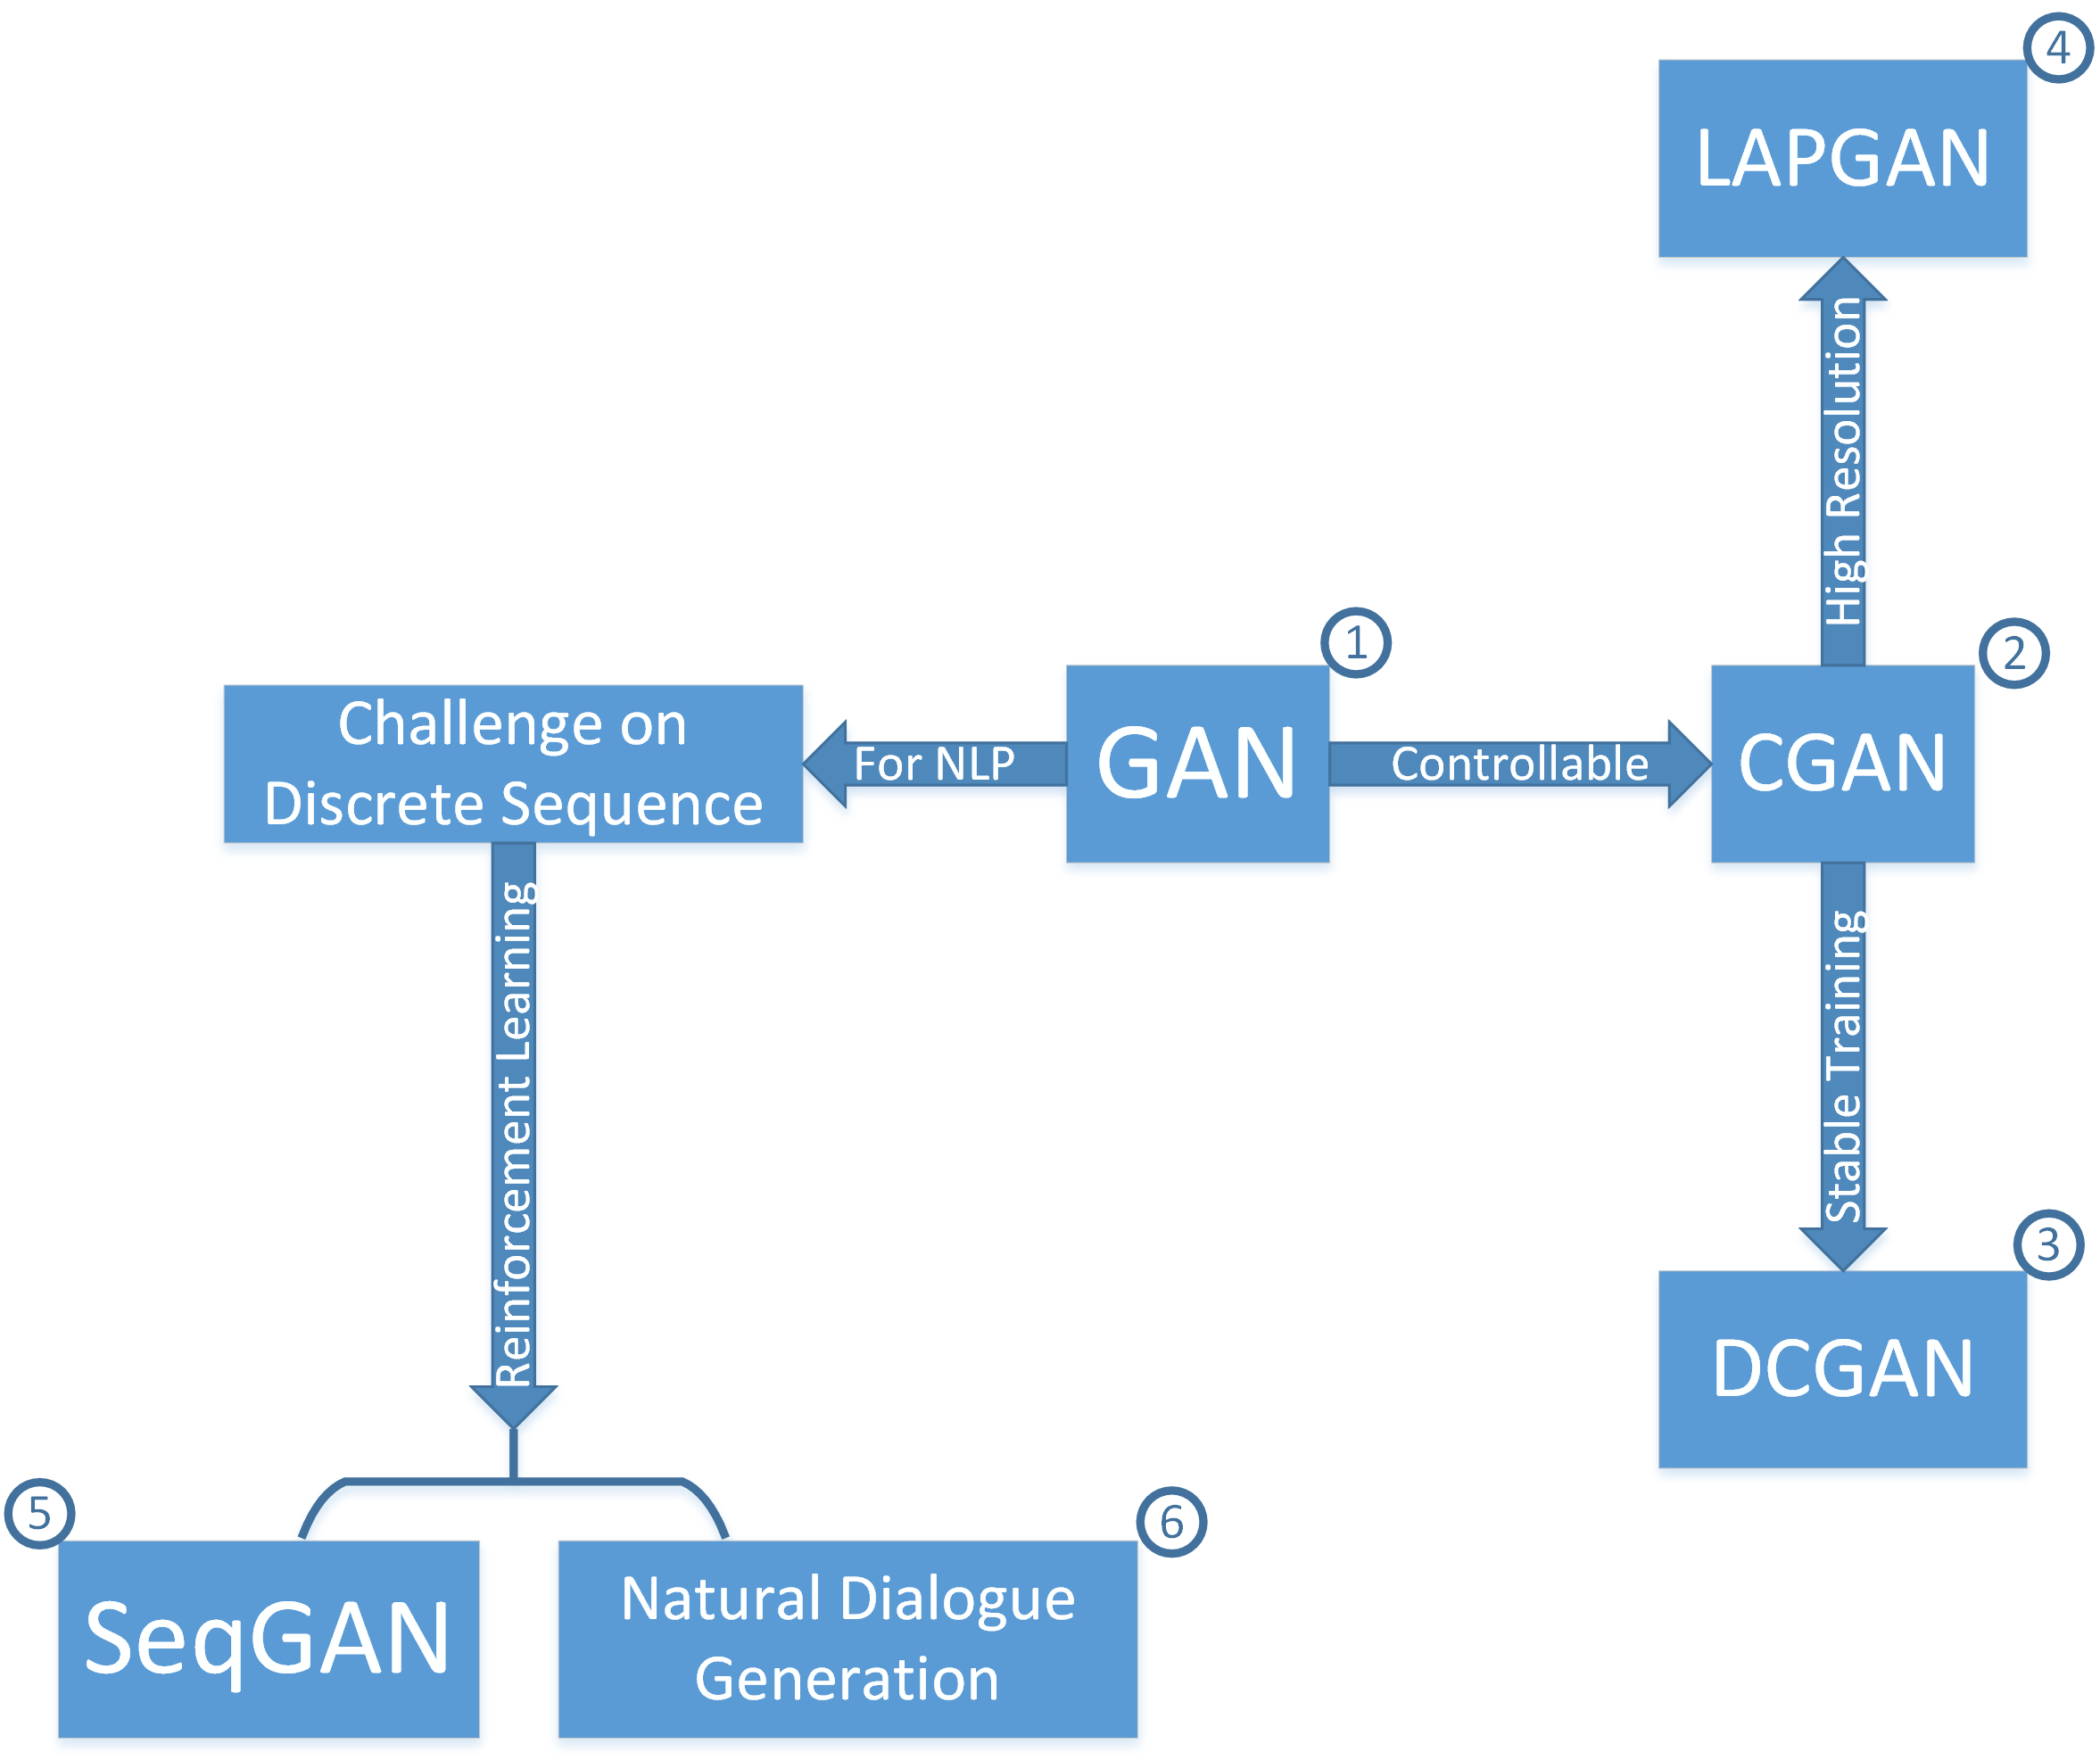
\includegraphics[width=25em]{figures/outline.png}
		\end{figure}
	\end{frame}
	\subtitlepage{}{Unsupervised Representation Learning with Deep Convolutional Generative Adversarial Networks}{Alec Radford, Luke Metz, Soumith Chintala\\arXiv: 1511.06434}
	\begin{frame}{Introduction}
		\begin{itemize}
			\item Shortcoming of GANs:
			\begin{itemize}
				\pause
				\item unstable to train
				\item nonsensical outputs.
			\end{itemize}
			\pause
			\item Very limited published research in trying to understand and visualize what GANs learn, and the intermediate representations of multi-layer GANs.
			\pause
			\item Contributions of this paper:
			\begin{itemize}
				\pause
				\item a set of constraints -> stable to train.
				\pause
				\item trained discriminators for image classification task -> competitive performance.
				\pause
				\item visualize the filters -> show that the filters learns to draw objects.
				\pause
				\item vector arithmetic properties -> semantic manipulation.
				\pause
			\end{itemize}
		\end{itemize}
	\end{frame}

	\begin{frame}{Approach}
		\begin{itemize}
			\item Architecture guidlines for stable Deep Convolution GANs:
			\begin{itemize}
				\pause
				\item Replace any pooling layers with strided convolutions (discriminator) and fractional-strided convolutions (generator).
				\pause
				\item Use batch normalization in both the generator and the discriminator.
				\pause
				\item Remove fully connected hidden layers for deeper architectures.
				\pause
				\item Use ReLU activation in generator for layers except for the output. which uses Tanh.
				\pause
				\item Use LeakyReLU activation in the discriminator for all layers.
			\end{itemize}
		\end{itemize}
	\end{frame}

	\begin{frame}{Structure}
		\begin{figure}
			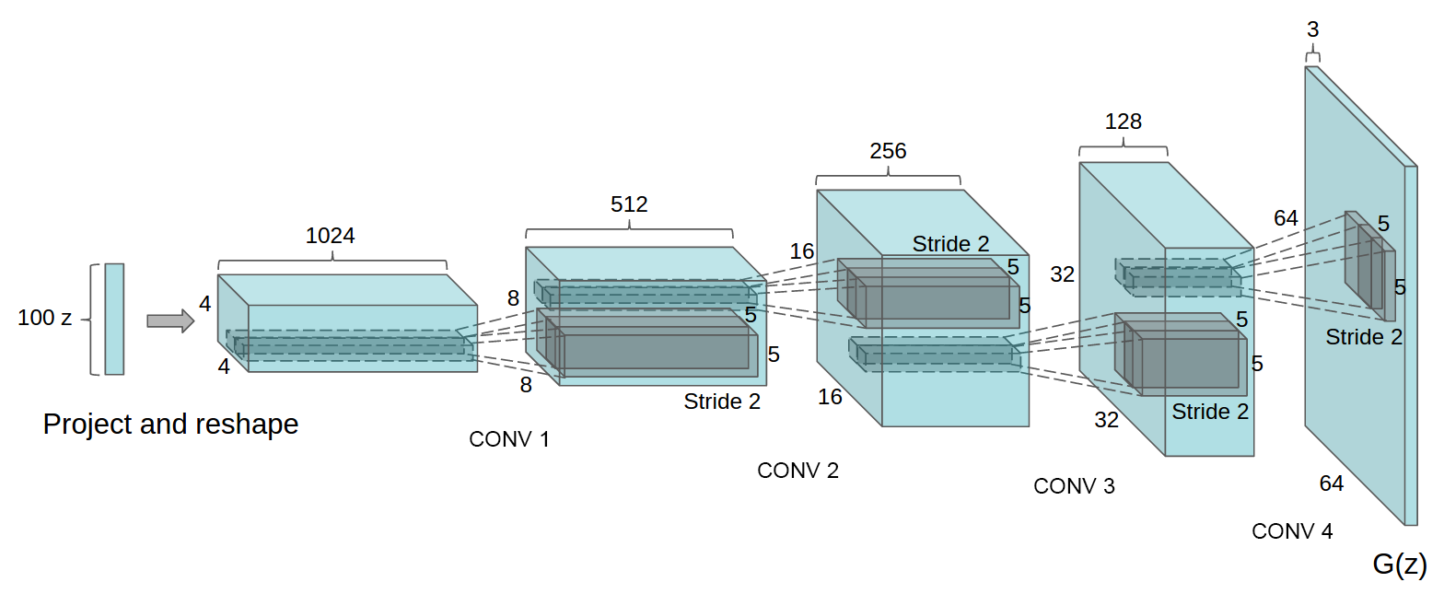
\includegraphics[width=25em]{figures/DCGAN-generator-structure.png}
			\caption{DCGAN generator used for LSUN scene modeling.}
		\end{figure}
		\pause
		During the training, many technics are adopted including dropout and momentum.
	\end{frame}

	\begin{frame}{Experiment}
		\begin{figure}
			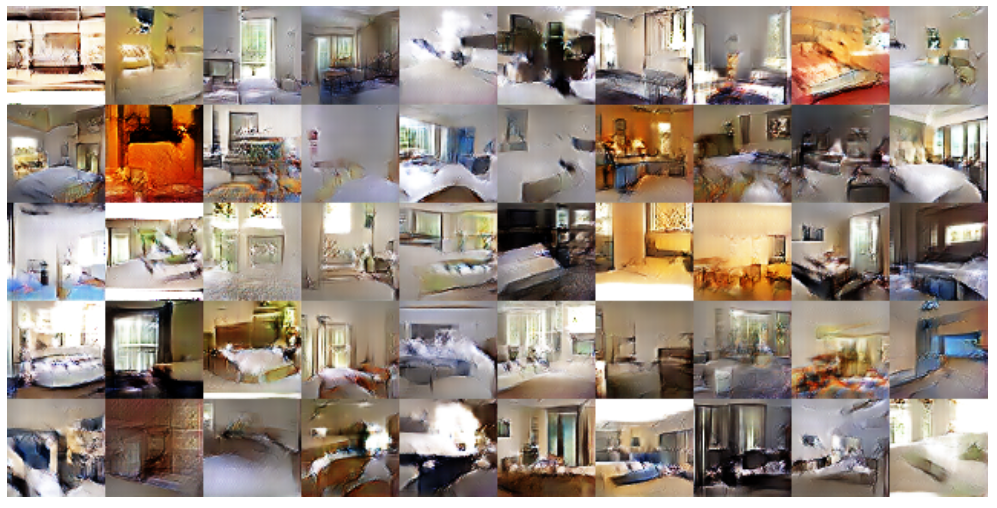
\includegraphics[width=23em]{figures/DCGAN-generated-image-epoch-1.png}
		\end{figure}
		\vspace{-1.5em}
		\begin{figure}
			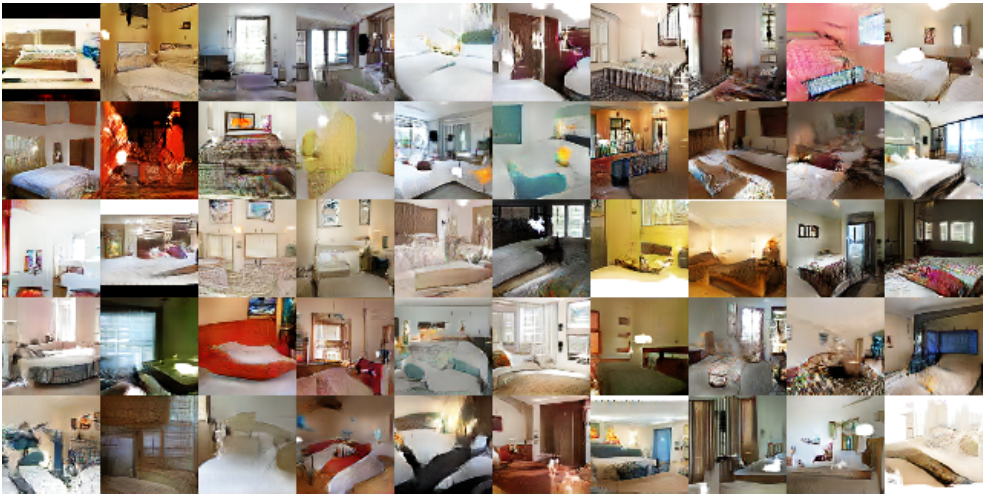
\includegraphics[width=23em]{figures/DCGAN-generated-image-epoch-5.png}
		\end{figure}
	\end{frame}

	\begin{frame}{Empirical Validation of DCGANs Capabilities}
		\begin{itemize}
			\pause
			\item Classifying CIFAR-10 using GANs as a Feature Extractor.
			\pause
			\item To evaluate the quality of the representations learnt by DCGANs for supervised tasks:
			\begin{itemize}
				\pause
				\item the model was trained on ImageNet-1k.
				\pause
				\item use the discriminator's convolutional features from all layers.
				\pause
				\item maxpooling each layers representation to produce a $4\times 4$ spatial grid.
				\pause
				\item flattened and concatenated to form a 28672 dimensional vector.
			\end{itemize}
			\begin{figure}
				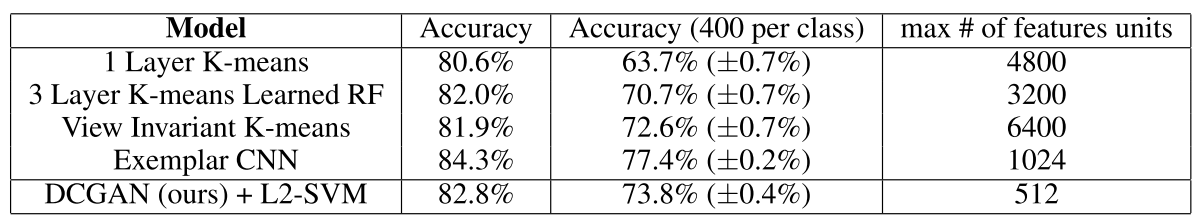
\includegraphics[width=30em]{figures/DCGAN-discriminator-feature-extractor-cifar-10.png}
			\end{figure}
		\end{itemize}
	\end{frame}

	\begin{frame}{Empirical Validation of DCGANs Capabilities}
		\begin{itemize}
			\item for StreetView House Numbers dataset (SVHN)
			\begin{figure}
				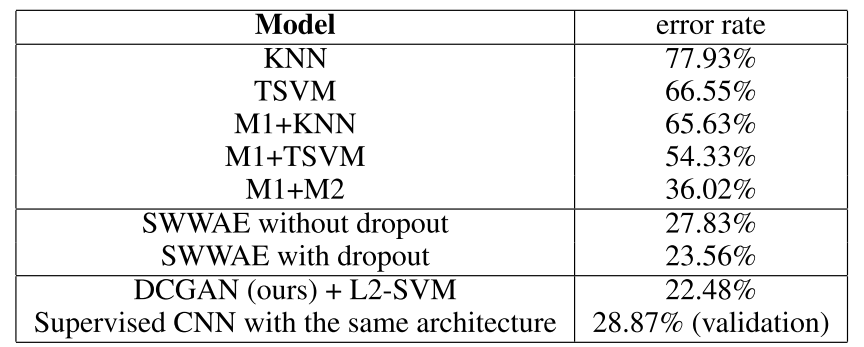
\includegraphics[width=15em]{figures/DCGAN-discriminator-feature-extractor-svhn.png}
			\end{figure}
			\pause
			\item L2-SVM classifier on the top of same feature extraction extraction pipeline used for CIFAR-10.
			\pause
			\item Achieves state of the art (for classification using 1000 labels) at 22.48\% test error.
			\pause
			\item Additionally, authors trained a purely supervised CNN with the same architecture on the same data -> CNN architecture used in DCGAN is not the key contributing factor of the model's performance.
		\end{itemize}
	\end{frame}

	\begin{frame}{Investigating and Visualizing the Internals of the Networks}
		\begin{itemize}
			\item How to prove that the model learned feature representation instead of the mapping from a noise to a sample?
			\pause
			\item If model learned the semantic representation, we can conduct small image transforms on feature space.
			\pause
			\item The first experiment was to understand the landscape of the latent space.
			\pause
			\item If walking in this latent space results in semantic changes to the image generations (such as object being added and removed), we can reason that the model has learned relevant and interesting representations.
		\end{itemize}
	\end{frame}

	\begin{frame}{Investigating and Visualizing the Internals of the Networks}
		\begin{figure}
			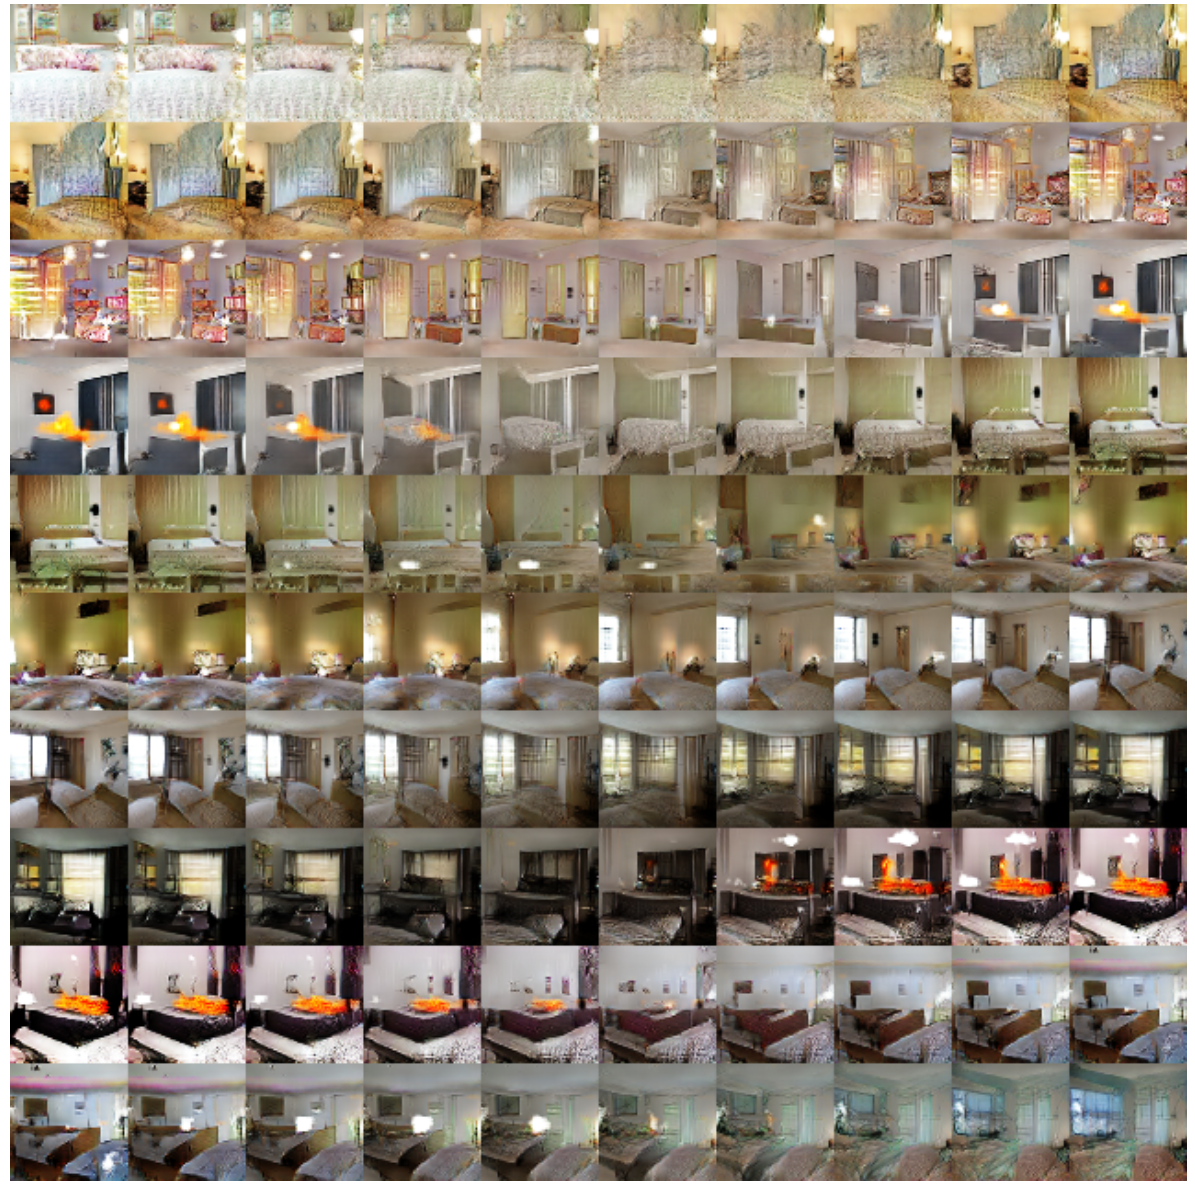
\includegraphics[width=23em]{figures/DCGAN-visualizing-internals-walking-in-latent.PNG}
		\end{figure}
	\end{frame}

	\begin{frame}{Investigating and Visualizing the Internals of the Networks}
		\begin{itemize}
			\onslide<1->
			\item Unsupervised DCGAN trained on a large image dataset can also learn a hierarchy of features that are interesting.
			\onslide<2->
			\begin{figure}
				\only<1>{\mbox{\phantom{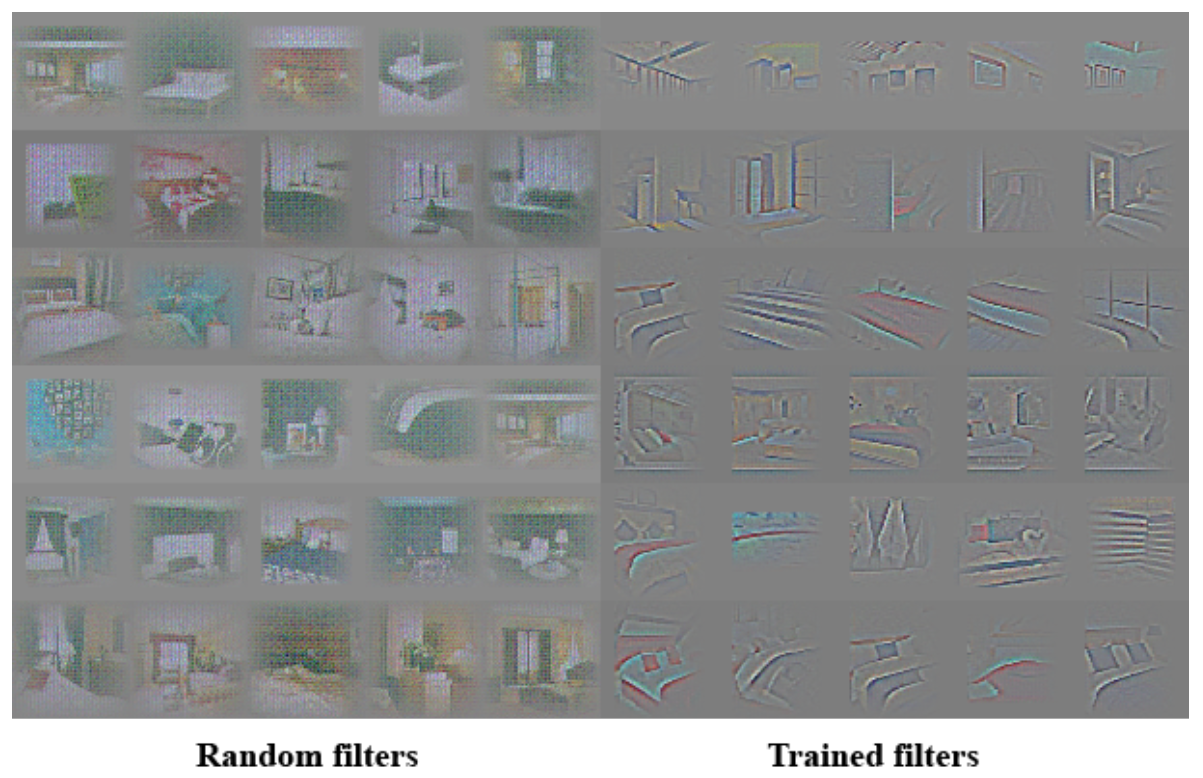
\includegraphics[width=25em]{figures/DCGAN-visualizing-internals-filters.png}}}}
				\includegraphics<2->[width=25em]{figures/DCGAN-visualizing-internals-filters.png}
				\caption{Features learnt by the discriminator.}
			\end{figure}
		\end{itemize}
	\end{frame}

	\begin{frame}{Investigating and Visualizing the Internals of the Networks}
		\begin{itemize}
			\item Manipulating the generator representation: Forgetting to draw certain objects.
			\pause
			\item What representations the generator learns? Scene components? Beds? Windows? Lamps? Doors?
			\pause
			\item If so, we can attempt to remove some component by manipulating the latent representation:
			\begin{itemize}
				\pause
				\item 150 samples, 52 window bounding boxes were drawn manually.
				\pause
				\item On the second highest convolution layers features, logistic regression was fit to predict whether a feature activation was on a window (or not).
				\pause
				\item by using the criterion that activations inside the drawn bounding boxes are positive and random samples from the same images are negatives.
				\pause
				\item All feature maps with weights greater than zero (200 in total) were dropped from all spatial locations.
				\pause
				\item Then, random new samples were generated with and without the feature map removal.
			\end{itemize}
		\end{itemize}
	\end{frame}

	\begin{frame}{Investigating and Visualizing the Internals of the Networks}
		\begin{figure}
			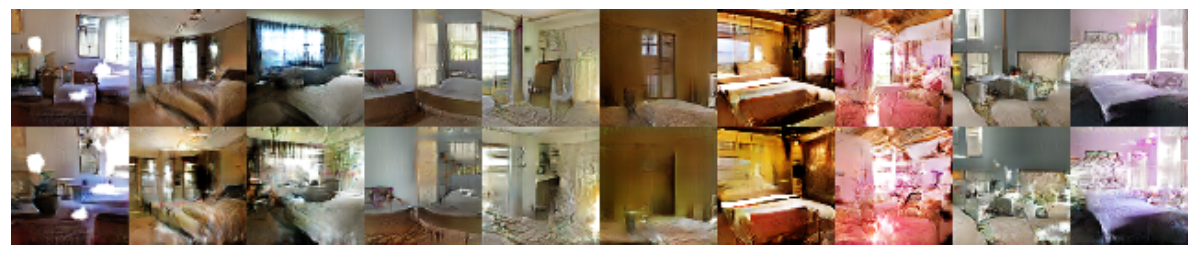
\includegraphics[width=30em]{figures/DCGAN-visualizing-internals-remove-filter.png}
		\end{figure}
		\begin{itemize}
			\item Top row: un-modified samples from model.
			\item Bottom row: the same samples generated with dropping out "window" filters.
			\item Some windows are removed, others are transformed into objects with similar visual appearance such as doors and mirrors.
		\end{itemize}
	\end{frame}
	
	\begin{frame}{Investigating and Visualizing the Internals of the Networks}
		\begin{itemize}
			\onslide<1->
			\item Representation of words: vector("King")-vector("Man")+vector("Woman")$\approx$vector("Queen").
			\onslide<2->
			\item Similar structure emerges in the $Z$ representation of generators.
			\onslide<3->
			\item Experiments working on only single samples per concept were unstable -> averaging the $Z$ vector for three examples.
			\onslide<4->
			\begin{figure}
				\only<1-3>{\mbox{\phantom{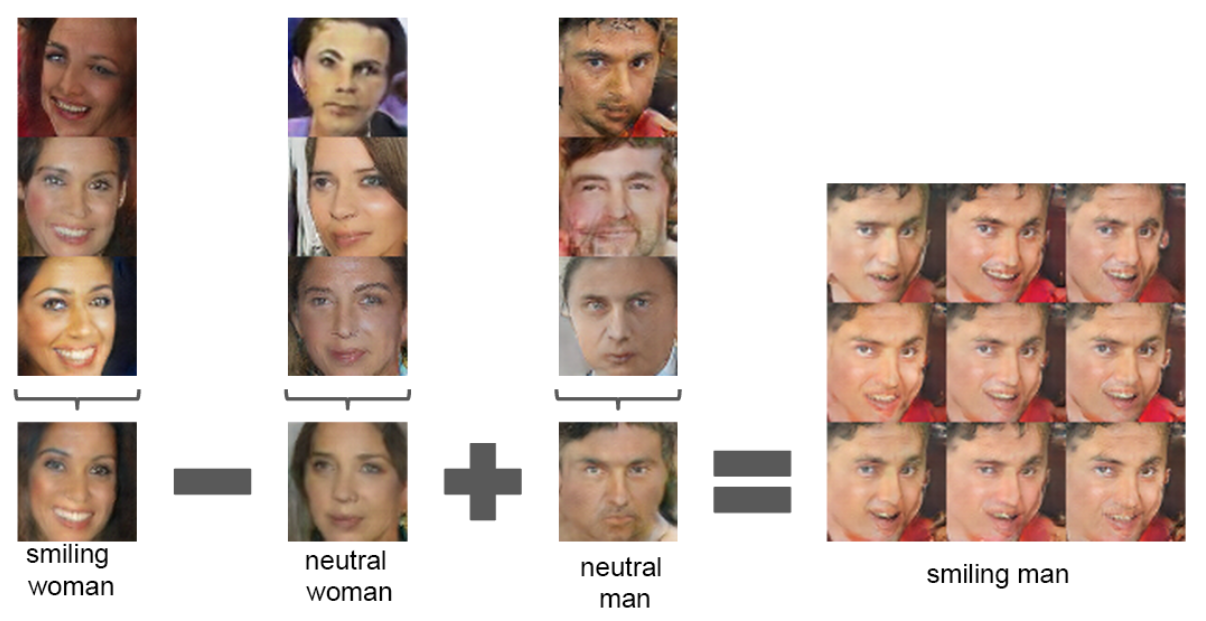
\includegraphics[width=25em]{figures/DCGAN-visualizing-internals-vector-1.PNG}}}}
				\includegraphics<4->[width=25em]{figures/DCGAN-visualizing-internals-vector-1.PNG}
			\end{figure}
		\end{itemize}
	\end{frame}

	\begin{frame}{Investigating and Visualizing the Internals of the Networks}
		\begin{figure}
			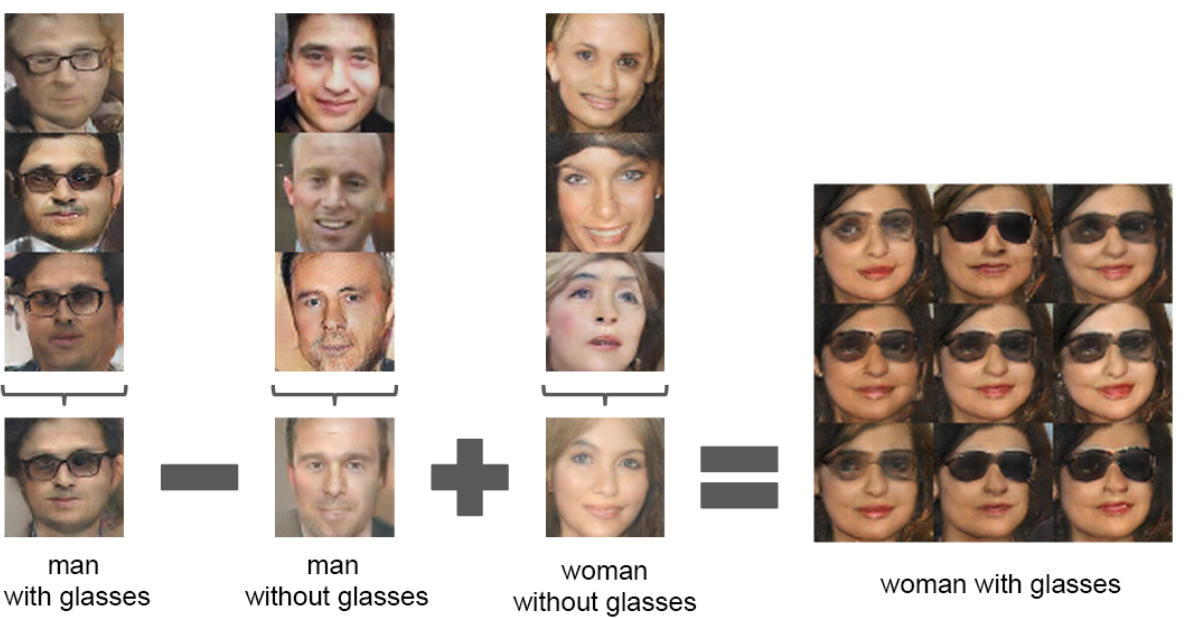
\includegraphics[width=25em]{figures/DCGAN-visualizing-internals-vector-2.PNG}
		\end{figure}
		\begin{figure}
			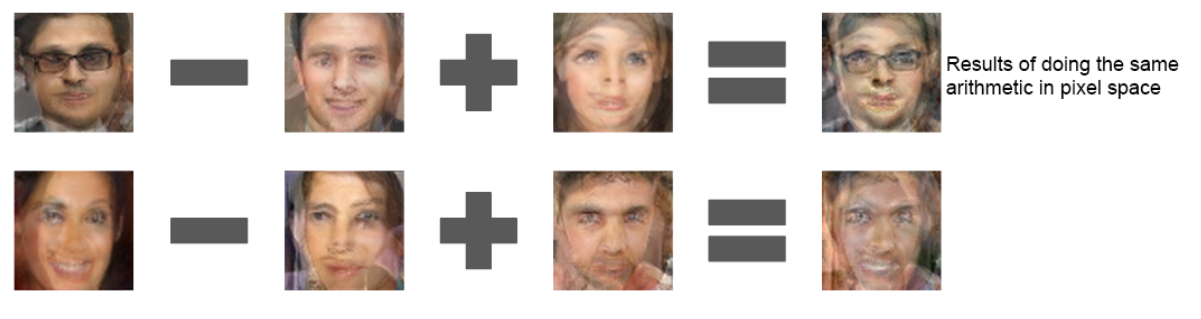
\includegraphics[width=25em]{figures/DCGAN-visualizing-internals-vector-3.PNG}
		\end{figure}
	\end{frame}

	\begin{frame}{Investigating and Visualizing the Internals of the Networks}
		\begin{figure}
			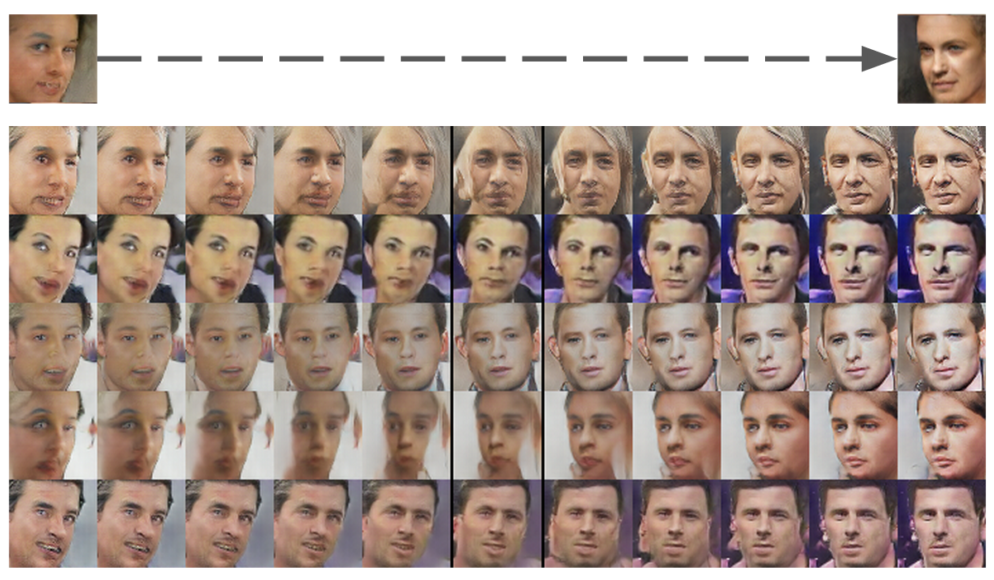
\includegraphics[width=25em]{figures/DCGAN-visualizing-internals-vector-4.PNG}
			\caption{A "turn" vector was created from four averaged samples of faces looking left vs looking right. By adding interpolations along this axis to random samples.}
		\end{figure}
	\end{frame}

	
	\part{LAPGAN}
	\begin{frame}{Outline}
		\begin{figure}
			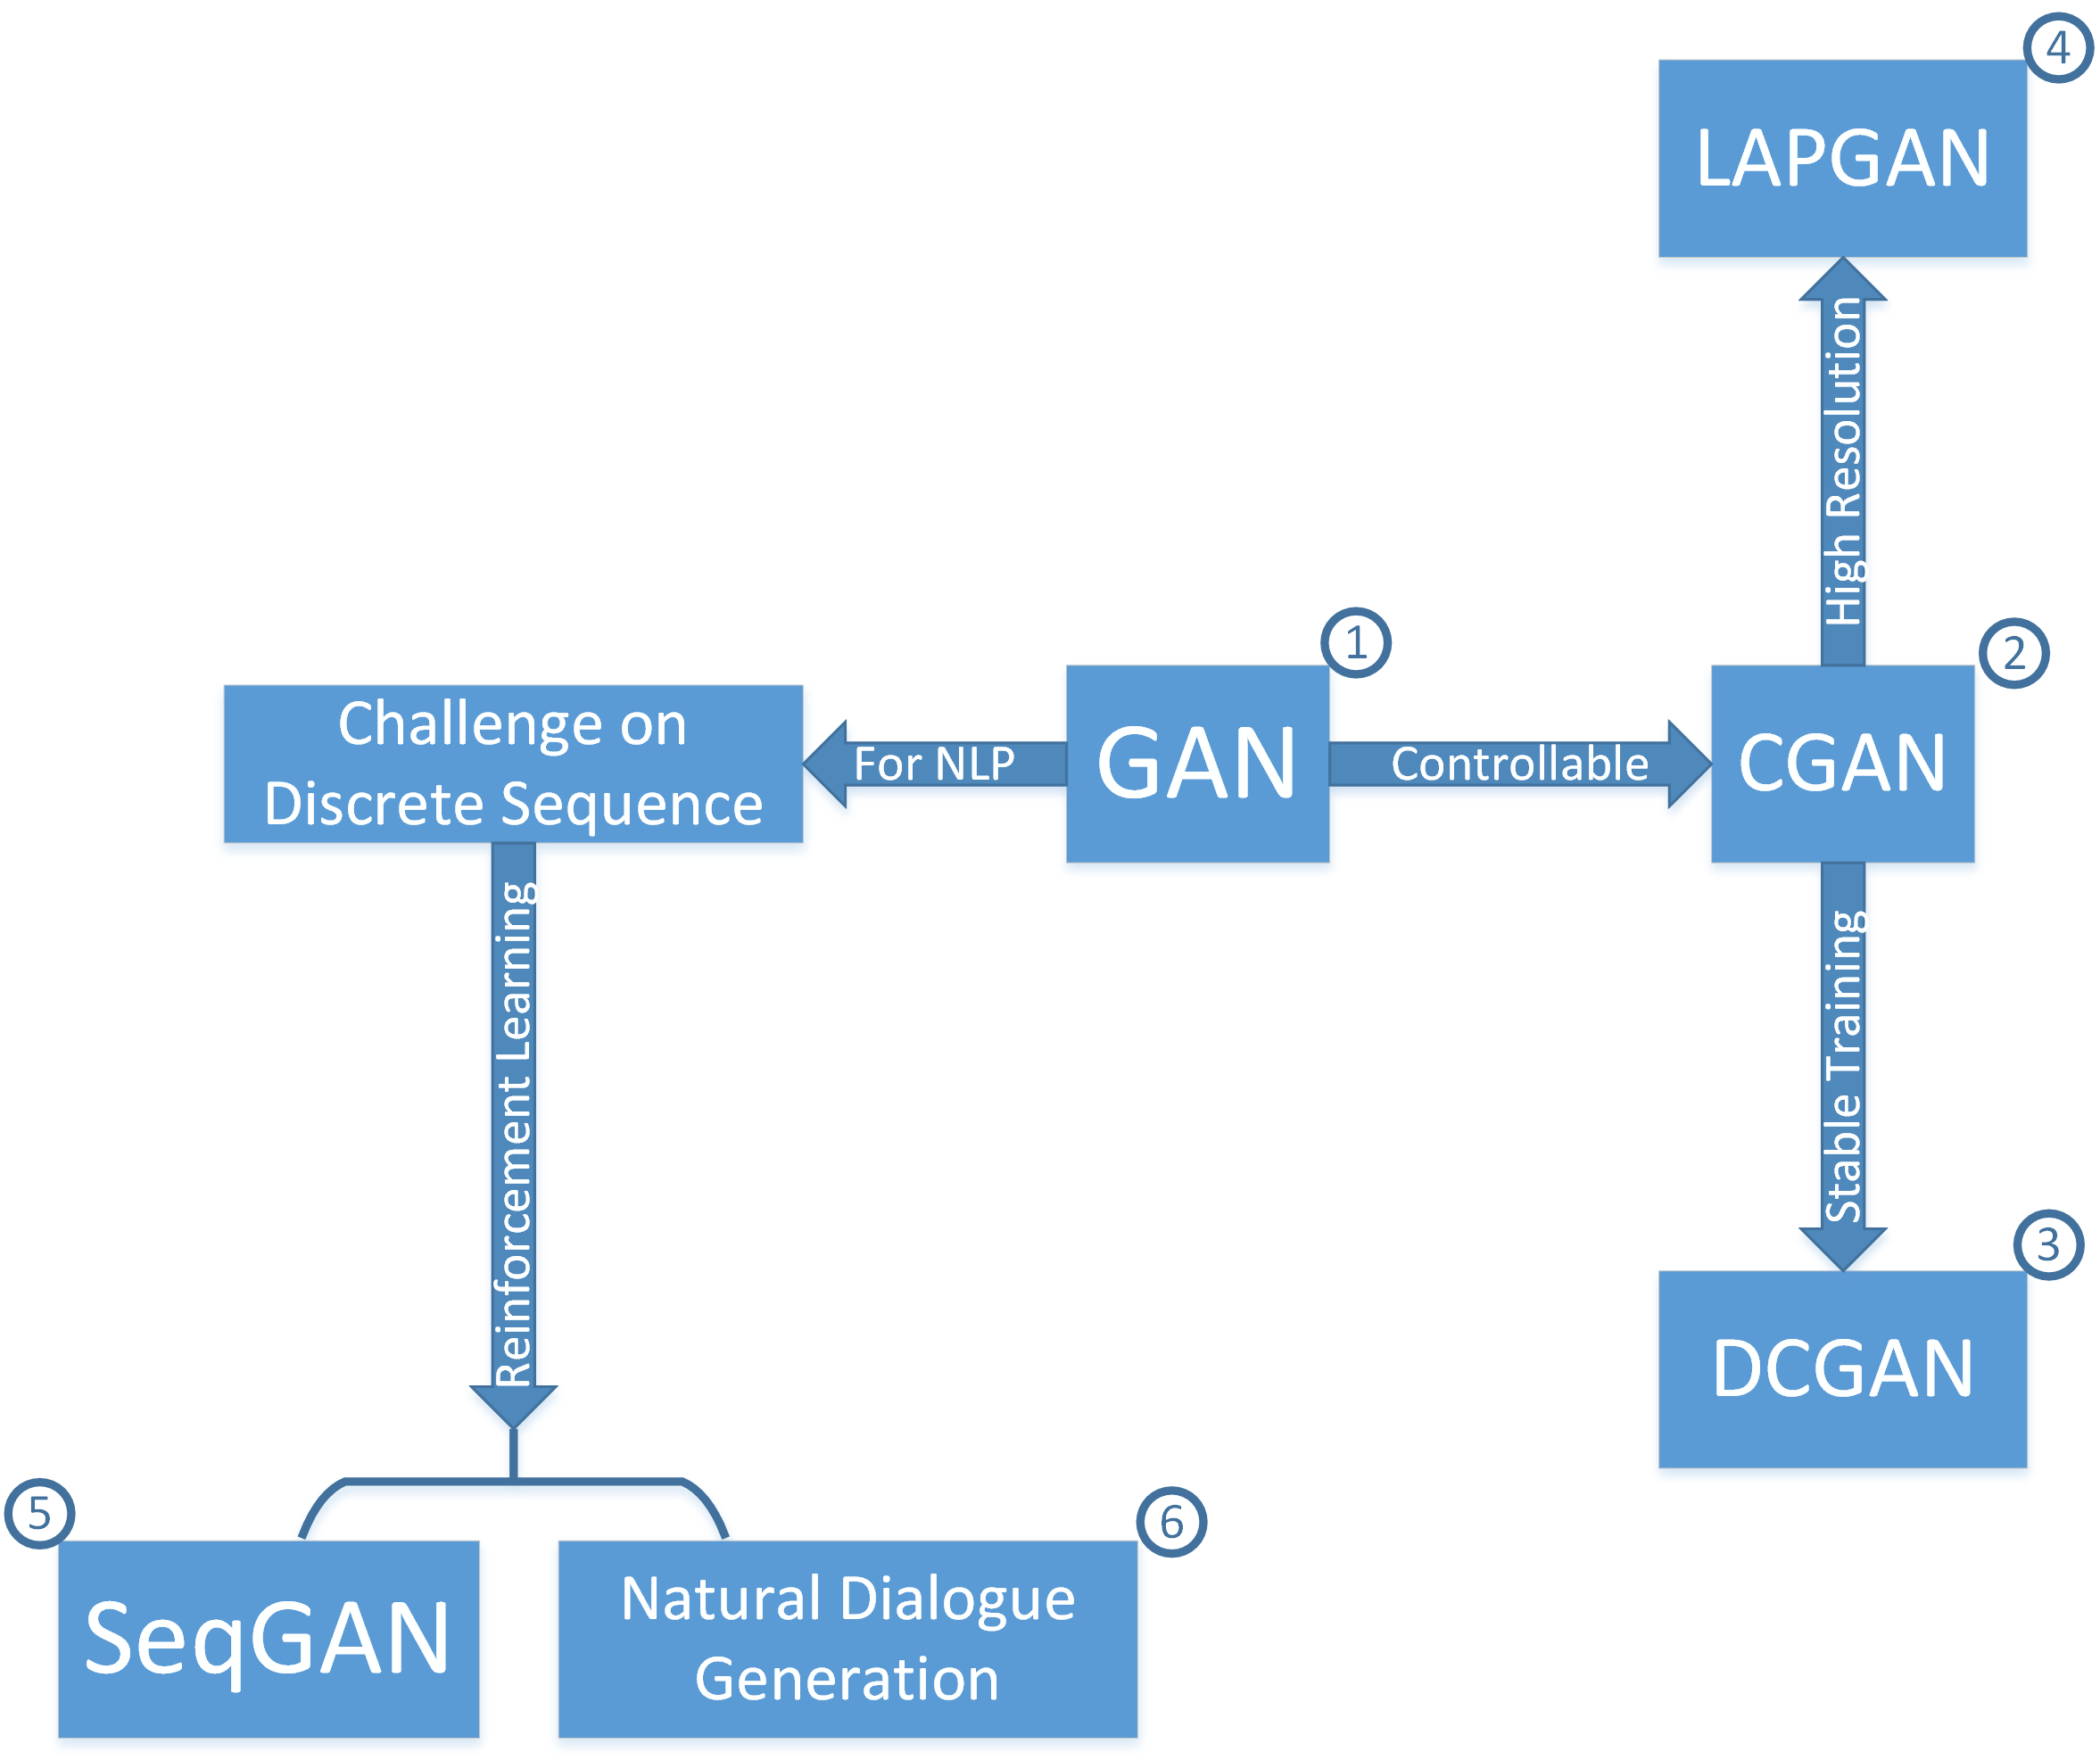
\includegraphics[width=25em]{figures/outline.png}
		\end{figure}
	\end{frame}
	\subtitlepage{}{Deep Generative Image Models using a Laplacian Pyramid of Adversarial Networks}{Emily Denton, Soumith Chintala, Arthur Szlam, Rob Fergus\\NIPS 2015\\arXiv: 1506.05751}
	
	\begin{frame}{Introduction}
		\begin{itemize}
			\item Building a good generative model of natural images has been a fundamental problem.
			\pause
			\item However, images are complex and high dimensional, making them hard to model well.
			\pause
			\item For the generation of high-resolution image, most existing approaches modelling entire scene instead generate image patches.
			\pause
			\item Multi-scale structure of natural images, building a series of generative models.
			\pause
			\item Each captures image structure at a particular scale of a Laplacian pyramid.
		\end{itemize}
	\end{frame}

	\begin{frame}{Laplacian Pyramid}
		\begin{itemize}
			\pause
			\item The main idea of Laplacian Pyramid is to consider the residue of the "image" and the "size-recovered down-sampled image".
			\pause
			\item If I is a $j\times j$ image.
			\pause
			\item Define $d(.)$ is down sampling. $d(I)$ will be a $j/2\times j/2$ image.
			\pause
			\item Define $u(,)$ is up sampling. $u(I)$ will be a $2j\times 2j$ image.
			\pause
			\item First build a Gaussian pyramid $\mathcal{G}(I)=[I_0,I_1,\dots,I_K]$.
			\pause
			\item $I_0=I$ and $I_k$ is $k$ repeated applications of $d(,)$. e.g. $I_2=d(d(I))$. $K$ is the number of levels in the pyramid.
			\pause
			\item The coefficient $h_k$ at each level $k$ of the Laplacian pyramid $\mathcal{L}(I)$ are constructed by taking the difference between adjacent levels in the Gaussian pyramid:
			\pause
			$$
			h_k=\mathcal{L}_k(I)=\mathcal{G}_k(I)-u(\mathcal{G}_{k+1}(I))=I_k-u(I_{k+1})
			$$
			\pause
			\item If we obtain, we can reconstruct the image from $I_K$ to $I_0$ by:
			\pause
			$$
			I_k=u(I_{k+1})+h_k
			$$
		\end{itemize}
	\end{frame}

	\begin{frame}{Laplacian Generative Adversarial Networks (LAPGAN)}
		\begin{itemize}
			\item LAPGAN followed these ideas by training a series of generators to build coefficients $\tilde{h}_k$ at each scale.
			\onslide<1->
			\item We can "draw" a high-resolution image by these coefficients by:
			\onslide<2->
			$$
			\tilde{I}_k=u(\tilde{I}_{k+1})+\tilde{h}_k=u(\tilde{I}_{k+1})+G_k(z_k,u(\tilde{I}_{k+1}))
			$$
			
			\onslide<3->
			\item The generative models ${G_0,\dots,G_k}$ are trained using the CGAN with the condition $u(\tilde{I}_{k+1})$ at each level of the pyramid.
			\onslide<4->
			\begin{figure}
				\only<1-3>{\mbox{\phantom{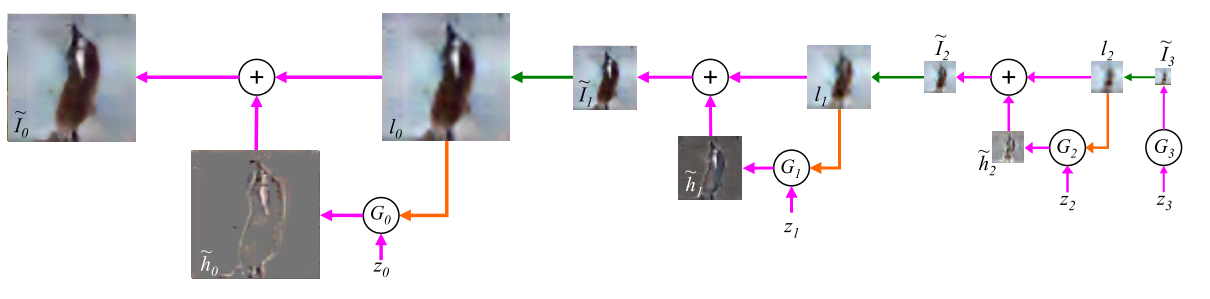
\includegraphics[width=30em]{figures/LAPGAN-generator-structure.png}}}}
				\includegraphics<4->[width=30em]{figures/LAPGAN-generator-structure.png}
				\caption{The structure of the generator of LAPGAN}
			\end{figure}
			\onslide<5->
			\item We will be able to calculate $\tilde{h}_k=G_k(z_k,u(I_{k+1}))$ and generate the high-solution realistic image if we have these GANs.
		\end{itemize}
	\end{frame}

	\begin{frame}{Laplacian Generative Adversarial Networks (LAPGAN)}
		\begin{itemize}
			\onslide<1->
			\item So, how do we get these GANs? (Training approach)
			\onslide<2->
			\begin{figure}
				\only<1>{\mbox{\phantom{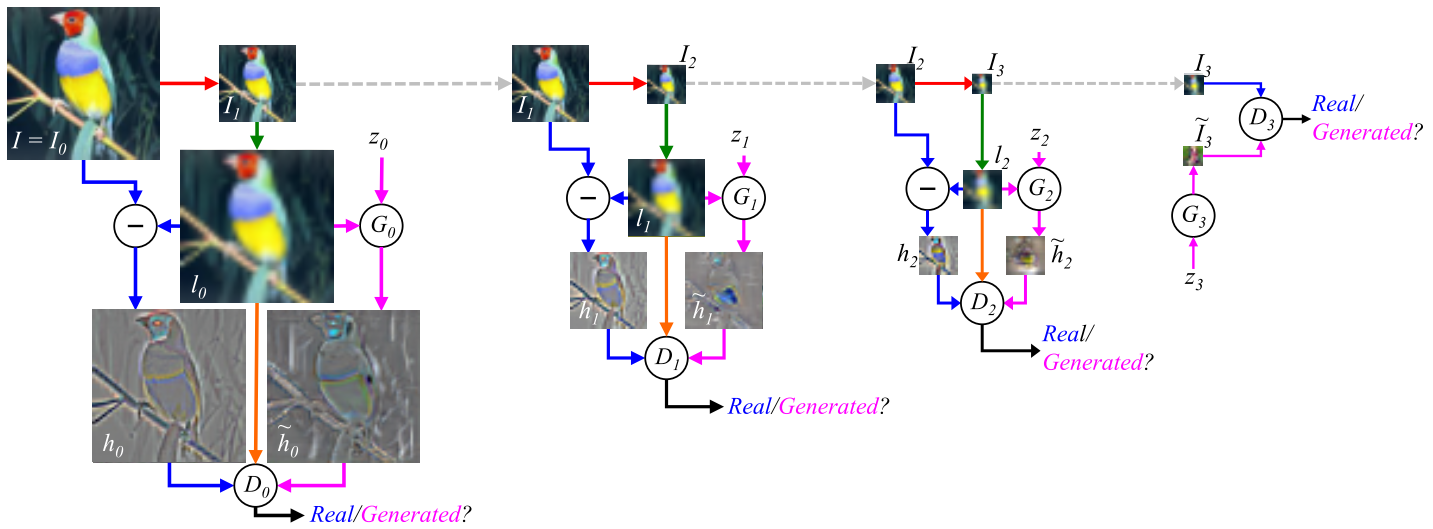
\includegraphics[width=25em]{figures/LAPGAN-general-structure.PNG}}}}
				\includegraphics<2->[width=25em]{figures/LAPGAN-general-structure.PNG}
				%\caption{The training procedure for LAPGAN model}
			\end{figure}
			\onslide<3->
			\item The training start with a $64\times64$ input image $I$ from trining set:
			\begin{enumerate}
				\onslide<4->
				\item take $I_0=I$ and down-sample it by a factor of two to produce $I_1$.
				\onslide<5->
				\item up-sample $I_1$ by a factor of two, giving a low-pass version $l_0$ of $I_0$.
				%\item with equal probability we use $l_0$ to create \emph{either} a real \emph{or} a generated example for the discriminative model $D_0$ that computes the probability of it being real vs generated.
				\onslide<6->
				\item In the real case (blue arrows), we compute high-pass $h_0=I_0-l_0$.
				\onslide<7->
				\item In the generated case (megenta arrows), the generative network $G_0$ receives as input a random noise vector $z_0$ and $l_0$. It outputs a generated high-pass image $\tilde{h}_0=G_0(z_0,l_0)$.
				\onslide<8->
				\item In both the real/generated cases, $D_0$ also receives $l_0$ as condition.
				\onslide<9->
				\item At level 3, $I_3$ is an $8\times8$ image, simple enough to be modeled directly with a standard GANs $G_3$ and $D_3$
			\end{enumerate}
		\end{itemize}
	\end{frame}

	\begin{frame}{Laplacian Generative Adversarial Networks (LAPGAN)}
		\begin{itemize}
			\item The key idea in this work is breaking the generation into successive refinements.
			\pause
			\item Give up any "global" manipulation.
			\pause
			\item Never make any attempt to train a network to discriminate between the output of a cascade and a real image and instead focus on making each step plausible.
			\pause
			\item Furthermore, the independent training of each pyramid level has the advantage that it is far more difficult for the model to memorize training examples --- a hazard when high capacity deep networks are used. (over-fit in generative model).
		\end{itemize}
	\end{frame}

	\begin{frame}{Experiment}
		\begin{figure}
			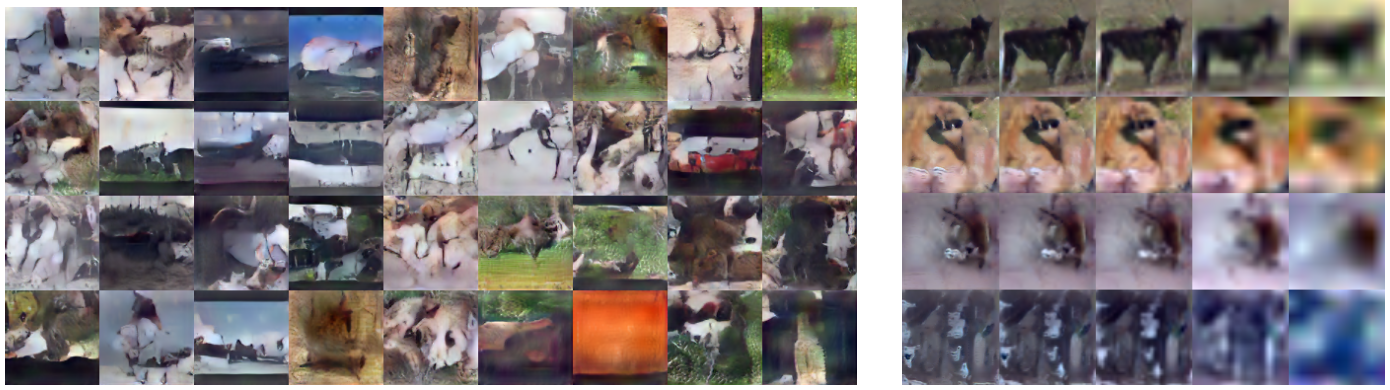
\includegraphics[width=30em]{figures/LAPGAN-experiment.png}
			\caption{STL 10 Samples: \\(a) Random $96\times96$ samples from our LAPGAN model. \\(b) Coarse-to-fine generation chain.}
		\end{figure}
	\end{frame}
	
	\part{GAN for Image Synthesis}
	\begin{frame}{Outline}
		\begin{figure}
			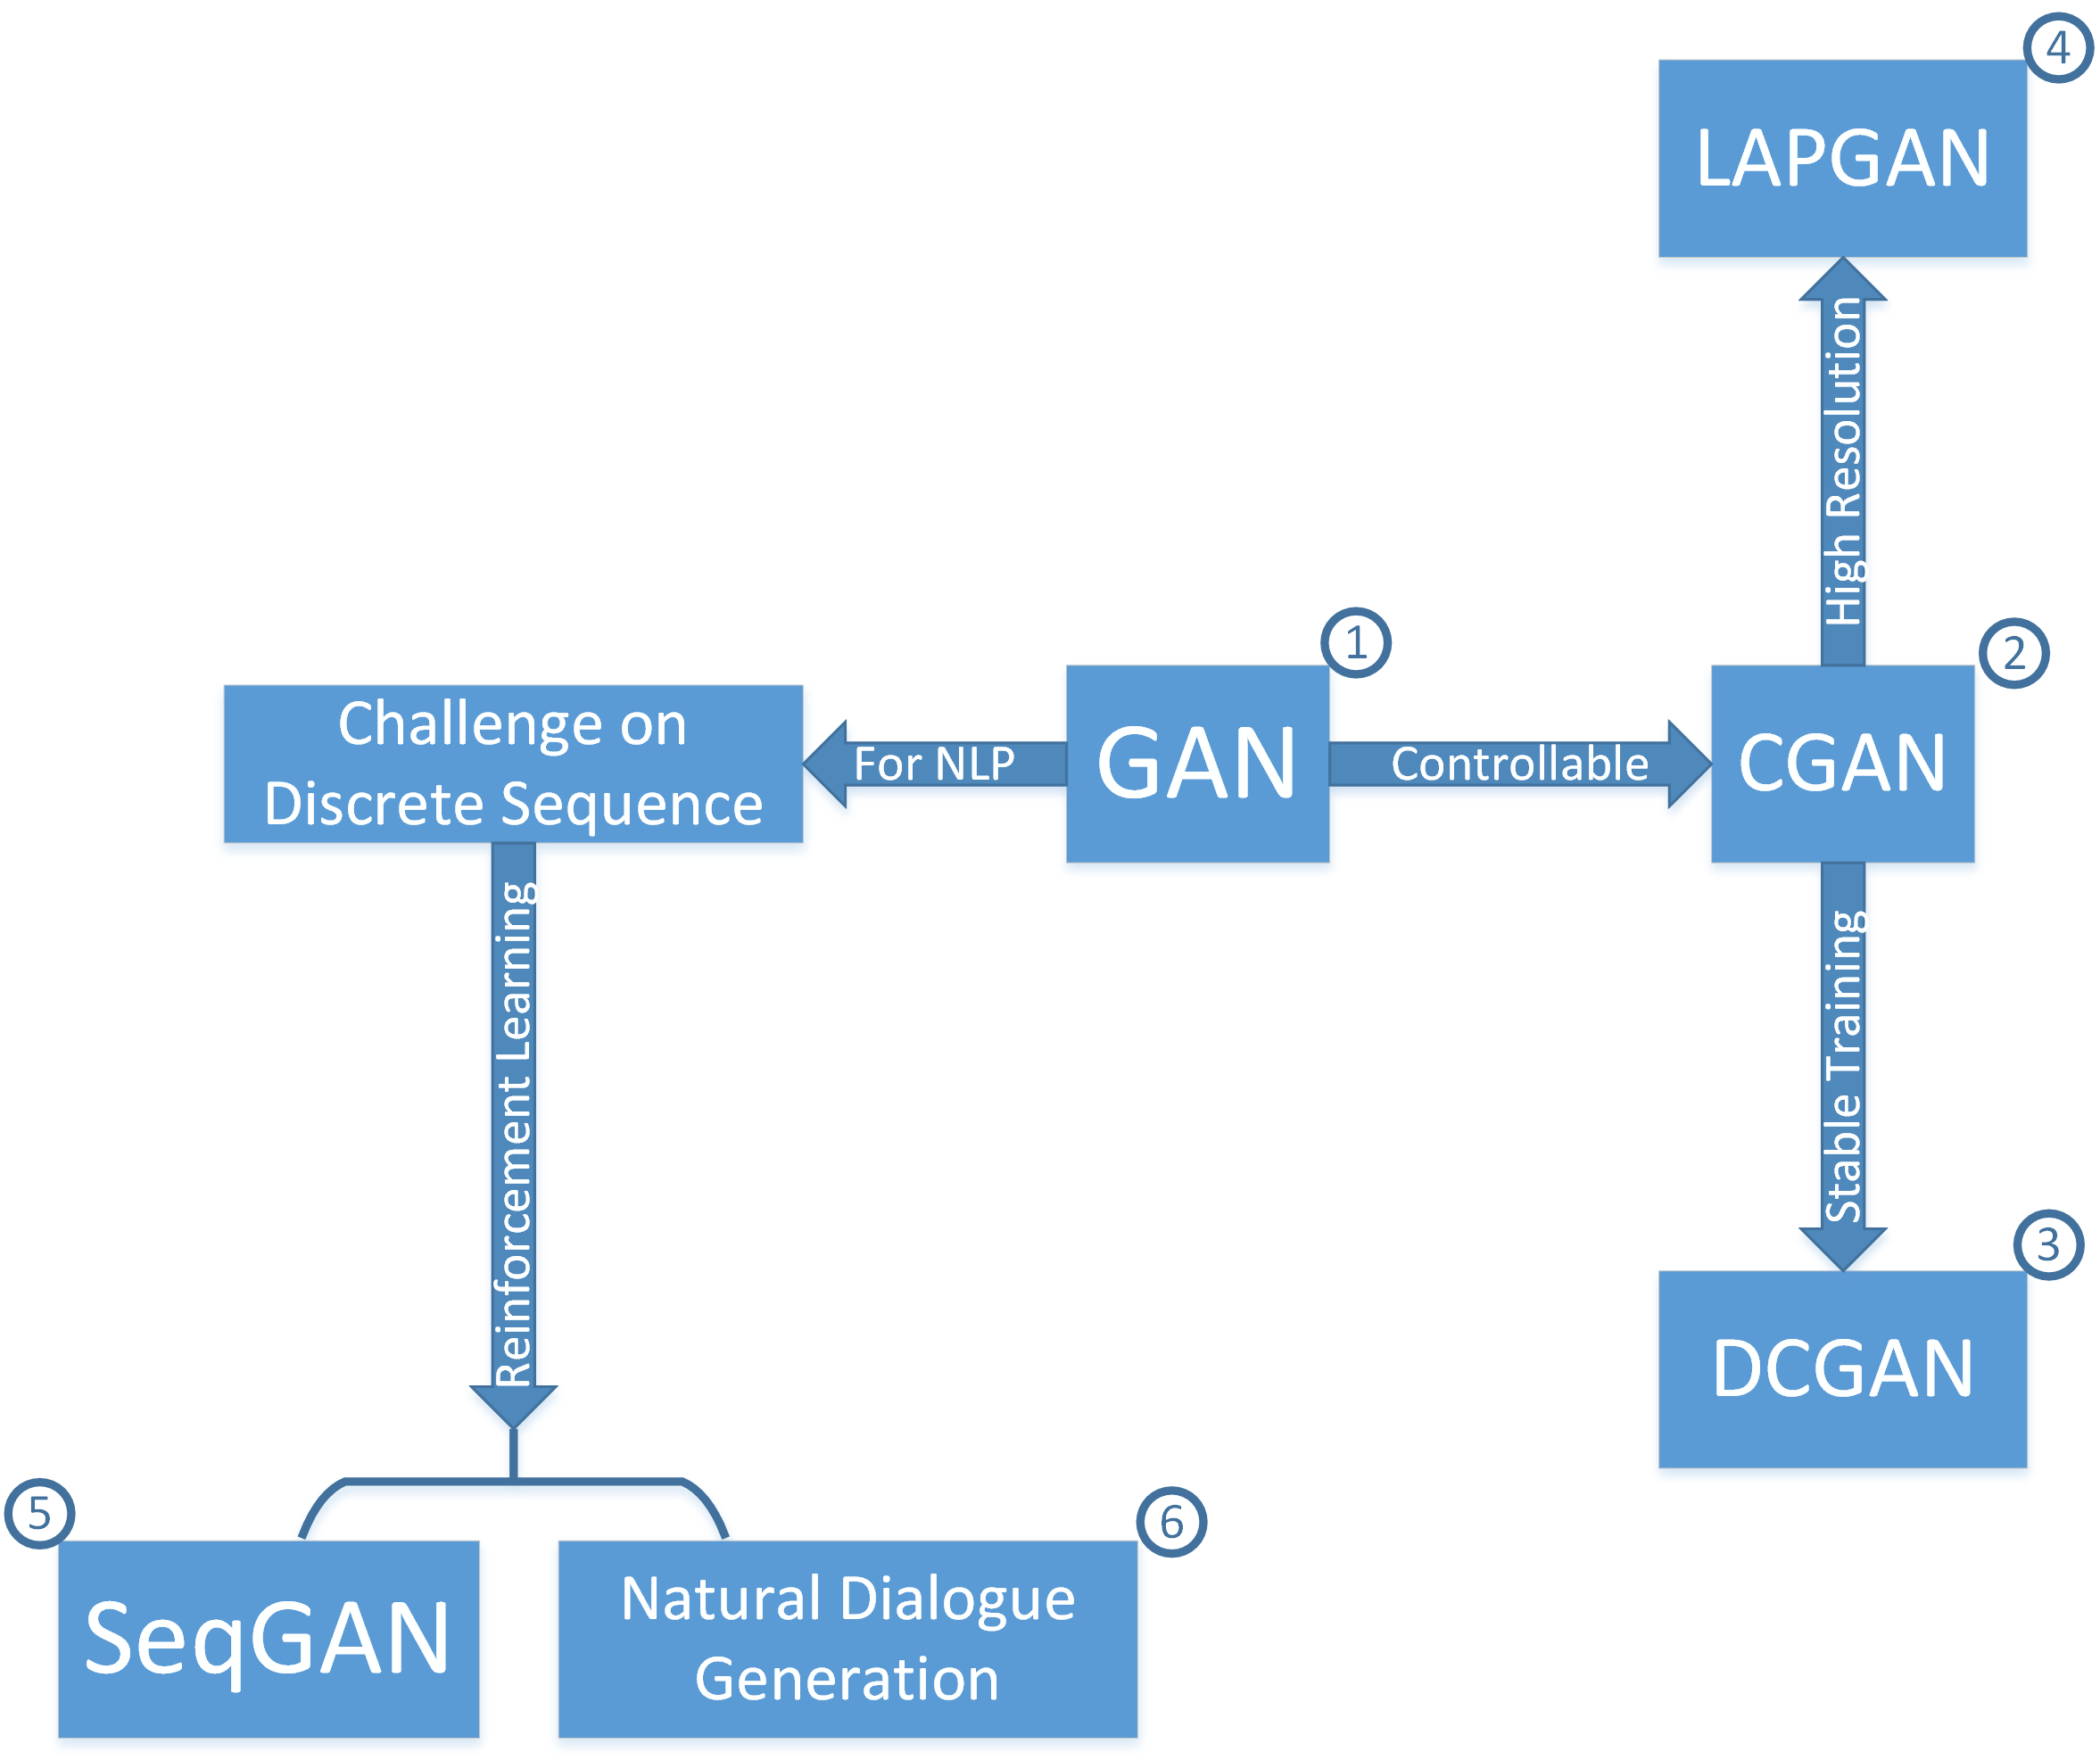
\includegraphics[width=25em]{figures/outline.png}
		\end{figure}
	\end{frame}
	\subtitlepage{}{Generative Adversarial Text to Image Synthesis}{Scott Reed, Zeynep Akata, Xinchen Yan, Lajanugen Logeswaran, Bernt Schiele, Honglak Lee\\ICML2016+JMLR Vol.48\\arXiv: 1605.05396}
	
	\begin{frame}{Introduction}
		\begin{itemize}
			\onslide<1->
			\item Papers we mentioned earlier are all about "generate realistic images".
			\onslide<2->
			\item Can we translat text in the form of single-sentence human-written descriptions directly into image pixels?
		\end{itemize}
		\onslide<3->
		\begin{figure}
			\only<1-2>{\mbox{\phantom{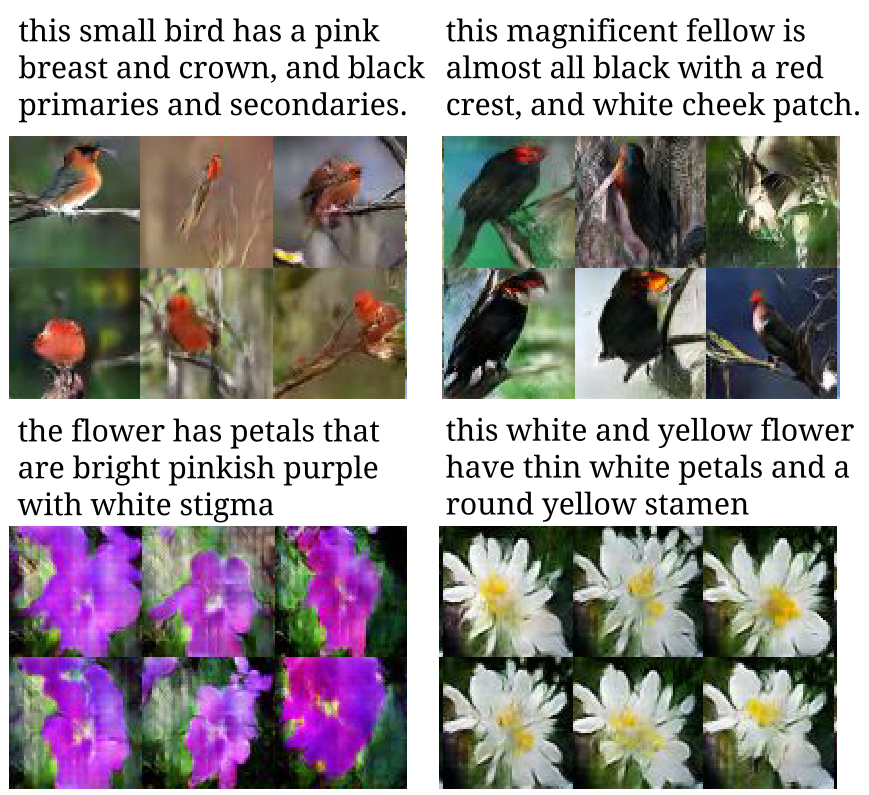
\includegraphics[width=17em]{figures/image-synthesis-prelude-demo.png}}}}
			\includegraphics<3->[width=17em]{figures/image-synthesis-prelude-demo.png}
		\end{figure}
	\end{frame}

	\begin{frame}{Introduction}
		\begin{itemize}
			\item This work aims to learn a mapping directly from words and characters to image pixels.
			\pause
			\item To solve this challenging problem requires solving two sub problems:
			\begin{enumerate}
				\pause
				\item learn a text feature representation that captures the important visual details
				\pause
				\item use these features to synthesize a compelling image that a human might mistake for real.
			\end{enumerate}
			\pause
			\item Fortunately, deep learning has enabled enormous progress in both sub problems - natural language representation and image synthesis.
			\pause
			\item This task will be build on these previous works.
		\end{itemize}
	\end{frame}

	\begin{frame}{Method}
		\begin{itemize}
			\onslide<1->
			\item Approach is to train a deep convolutional generative adversarial network (DCGAN) conditioned on text features encoded by a hybird character-level convolutional-recurrent neural network.
			\onslide<2->
			\item Both the generator network $G$ and the discriminator network $D$ perform feed-forward inference conditioned on the text feature.
			\onslide<3->
			\item The generator network is denoted $G$: $\mathrm{R}^Z\times\mathrm{R}^T\rightarrow\mathrm{R}^D$.
			\onslide<4->
			\item The discriminator as $D$: $\mathrm{R}^D\times\mathrm{R}^T\rightarrow{0,1}$.
			\onslide<5->
			\item $T$ is the dimension of the text description embedding, $D$ is the dimension of the image, and $Z$ is the dimension of the noise input to $G$.
		\end{itemize}
		\onslide<6->
		\begin{figure}
			\only<1-5>{\mbox{\phantom{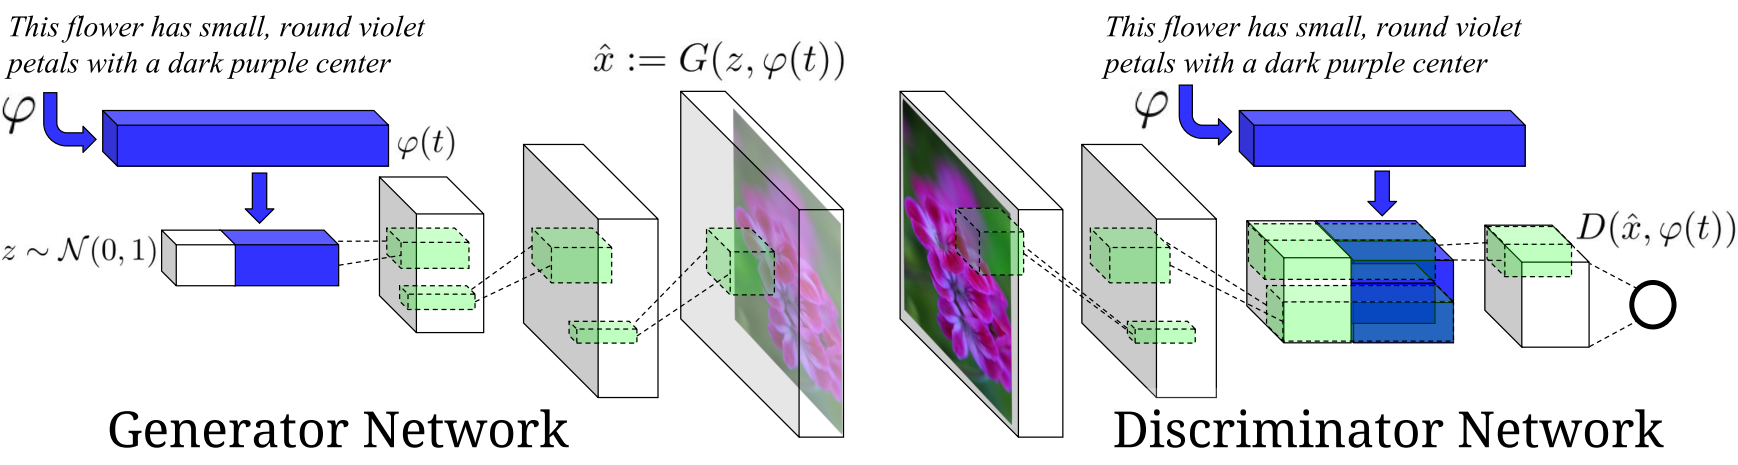
\includegraphics[width=30em]{figures/image-synthesis-structure.png}}}}
			\includegraphics<6->[width=30em]{figures/image-synthesis-structure.png}
		\end{figure}
	\end{frame}

	\begin{frame}[t]{Method}
		\begin{figure}
			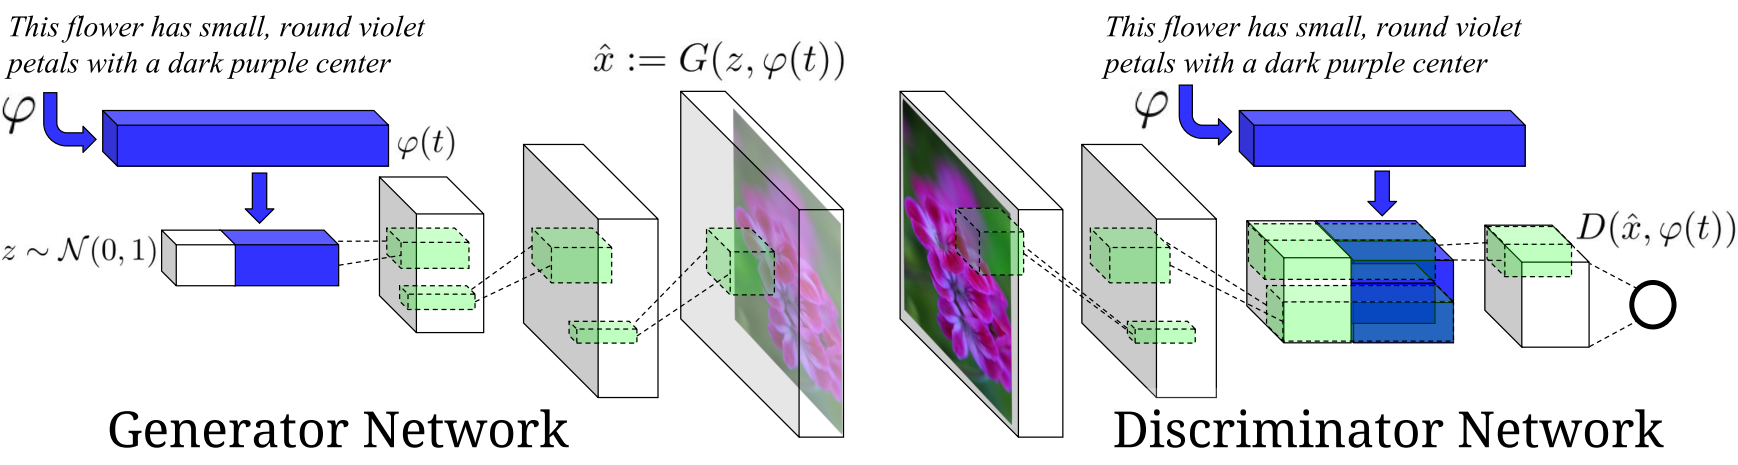
\includegraphics[width=30em]{figures/image-synthesis-structure.png}
		\end{figure}
		\begin{itemize}
			\pause
			\item in the generator $G$, sample from the noise prior $z\in\mathrm{R}^Z\sim\mathcal{N}(0,1)$
			\pause
			\item encode the text query $t$ using text encoder $\phi$.
			\pause
			\item the description embedding $\phi(t)$ is first compressed using a fully-connected layer to a small dimension followed by leaky-ReLU and then concatenated to the noise vector $z$.
			\pause
			\item inference proceeds as in a normal deconvolutional network: feed-forward it through the generator $G$; a synthetic image $\hat{x}$ is generated via $\hat{x}\leftarrow G(z,\phi(t))$.
		\end{itemize} 
	\end{frame}

	\begin{frame}[t]{Method}
		\begin{figure}
			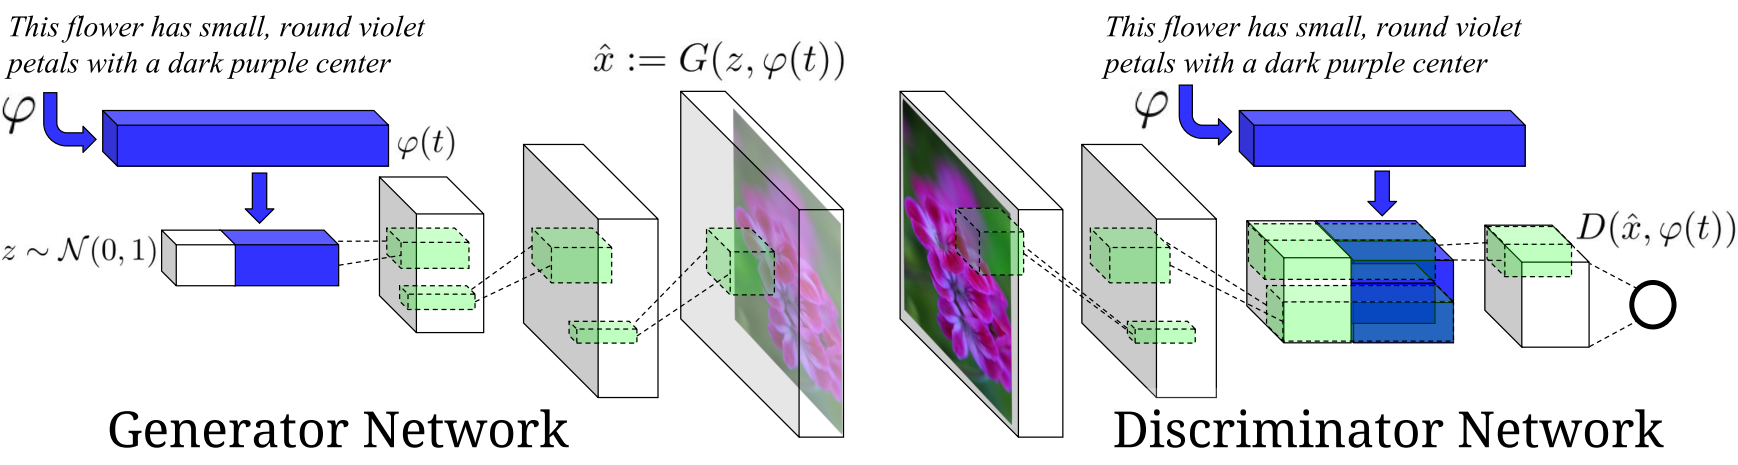
\includegraphics[width=30em]{figures/image-synthesis-structure.png}
		\end{figure}
		\begin{itemize}
			\item in the discriminator $D$, perform several layers of stride-2 convolution with spatial batch normalization followed by leaky ReLU.
			\pause
			\item replicate the description embedding spatially and perform a depth concatenation.
			\pause
			\item perform a $1\times1$ convolution followed by rectification and a $4\times4$ convolution to conpute the final score from $D$.
			\pause
			\item batch normalization is performed on all convolutional layers.
		\end{itemize}
	\end{frame}
	
	\begin{frame}{Training: GAN-CLS}
		\begin{itemize}
			\pause
			\item The most straightforward way to train a conditional GAN is to view (text, image) pairs as joint observation and train the discriminator to judge pairs as real or fake.
			\pause
			\item The discriminator has no explicit notion of whether real training images match the text embedding context.
			\pause
			\item The dynamics of learning may be different from the non-conditional case.
			\pause
			\item In naive GAN, the discriminator observes two kinds of inputs: real images with matching text, and synthetic images with arbitrary text.
			\pause
			\item It must implicitly separate two sources of error:
			\begin{enumerate}
				\pause
				\item unrealistic images (for \emph{any} text)
				\pause
				\item realistic images of the wrong class that mismatch the conditioning information.
			\end{enumerate}
		\end{itemize} 
	\end{frame}

	\begin{frame}{Training: GAN-CLS}
		\begin{itemize}
			\item Algorithm following summarizes the training procedure.
			\pause
			\begin{algorithm}[H]
				\algsetup{linenosize=\tiny}
				%\scriptsize
				\footnotesize
				\caption*{\textbf{Algorithm} \footnotesize GAN-CLS training algorithm with step size $\alpha$, using minibatch SGD for simplicity.}
				\begin{algorithmic}
					\pause
					\REQUIRE minibatch images $x$, matching text $t$, mismatching $\hat{t}$, number of training batch steps $S$
					\pause
					\FOR{$n=1,\dots,S$}
						\pause
						\STATE $h\leftarrow\phi(t)$ //encode matching text description
						\pause
						\STATE $\hat{h}\leftarrow\phi(\hat{t})$ //encode mis-matching text description
						\pause
						\STATE $z\sim\mathcal{N}(0,1)^Z$ //draw sample of random noise
						\pause
						\STATE $\hat{x}\leftarrow G(z,h)$ //forward through generator
						\pause
						\STATE $s_r\leftarrow D(x,h)$ // real image, right text
						\pause
						\STATE $s_w\leftarrow D(x,\hat{h})$ // real image, wrong text
						\pause
						\STATE $s_f\leftarrow D(\hat{x},h)$ // fake image, right text
						\pause
						\STATE $\mathcal{L}_D\leftarrow\log(s_r)+(\log(1-s_w)+log(1-s_f))/2$  
						\pause
						\STATE $D\leftarrow D-\alpha\partial\mathcal{L}_D/\partial D$ // update discriminator
						\pause
						\STATE $\mathcal{L}_G\leftarrow\log(s_f)$
						\pause
						\STATE $G\leftarrow G-\alpha\partial\mathcal{L}_G/\partial G$ // update generator
					\ENDFOR
				\end{algorithmic}
			\end{algorithm}
		\end{itemize}
	\end{frame}

	\begin{frame}{Training: GAN-INT}
		\begin{itemize}
			\item Sometimes, we can generate a large amount of additional text embeddings by simply interpolating between embeddings of training set.
			\pause
			\item These interpolated text embeddings need not correspond to any actual human-written text, so there is no additional labelling cost.
			\pause
			\item This can be viewed as adding an additional term to the generator objective to minimize:
			$$
			\mathrm{E}_{t_1,t_2\sim p_{\text{data}}}\left[\log(1-D(G(z,\beta t_1+(1-\beta)t_2)))\right]
			$$
		\end{itemize}
	\end{frame}

	\begin{frame}{Experiment}
		\begin{figure}
			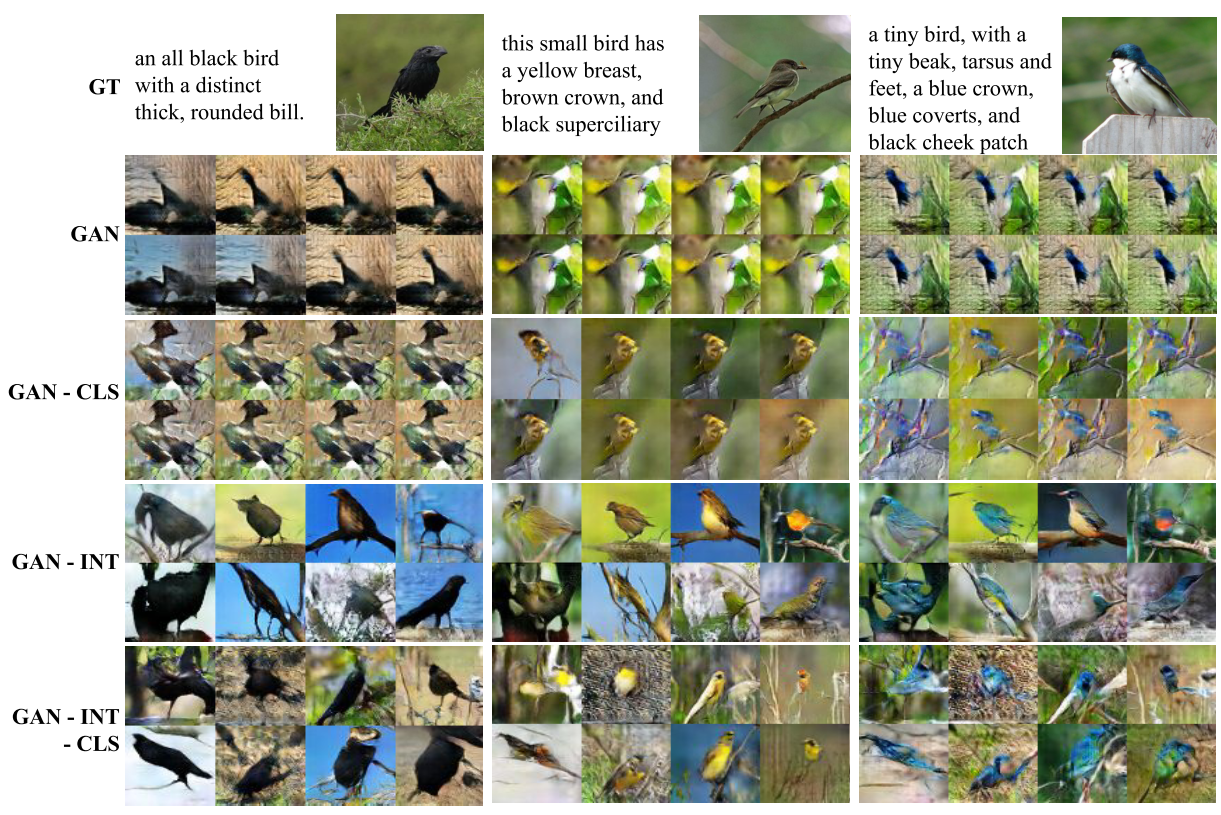
\includegraphics[width=30em]{figures/image-synthesis-experiment.PNG}
		\end{figure}
	\end{frame}
	
	\part{Challenges of GANs on NLP}
	\begin{frame}{Outline}
		\begin{figure}
			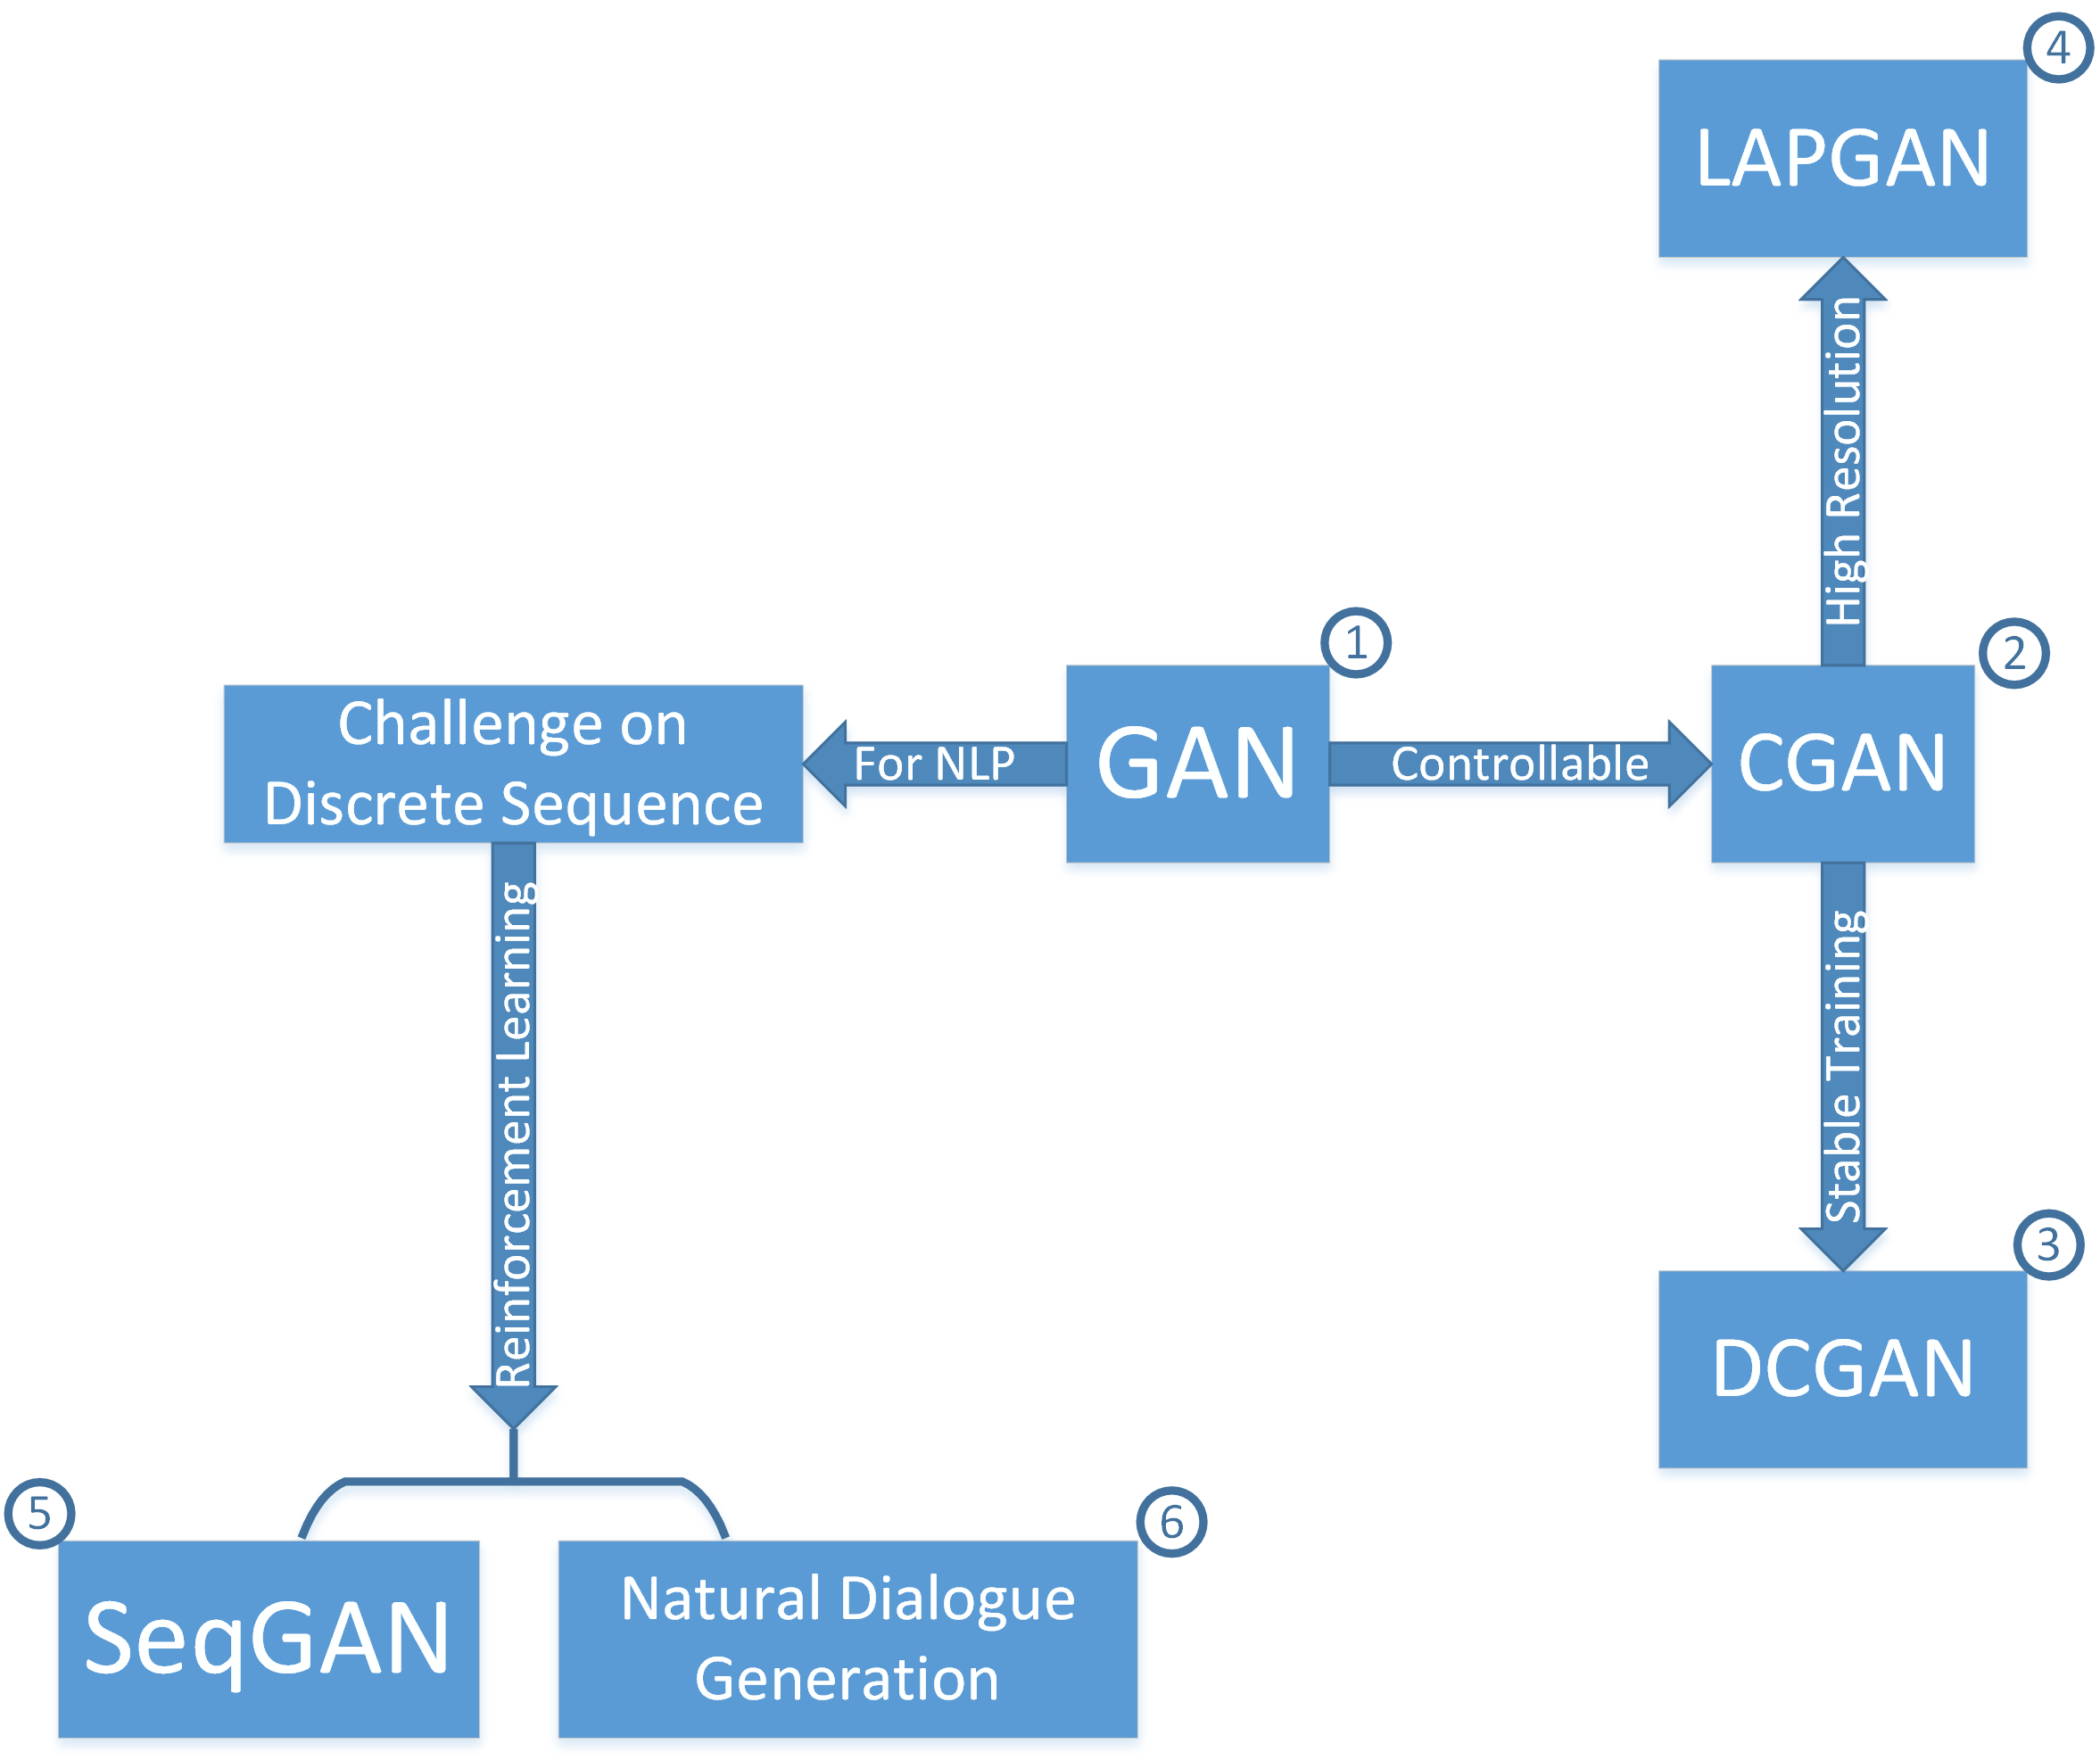
\includegraphics[width=25em]{figures/outline.png}
		\end{figure}
	\end{frame}
	\subtitlepage{}{Challenges of GANs on NLP}{}
	\begin{frame}{Challenges of GANs on NLP}
		\begin{itemize}
			\pause
			\item GAN are only defined for real-valued data. (pixels of an image, energy of audio frame.)
			\pause
			\item You can make slight changes to the synthetic data only if it is based on continuous numbers. If it is based on discrete numbers, there is no way to make a slight change.
			\pause
			\item E.g. $\text{pixel}(1.0)\approx\text{pixel}(1.00001)$. $\text{one-hot}(\text{penguin})\neq\text{one-hot}(\text{penguin+0.001})$
			\pause
			\item GAN can only give the score/loss for an entire sequence when it has been generated.
			\pause
			\item For a partially generated sequence, it is non-trivial to balance how good as it is not and the future score as the entire sequence.
		\end{itemize}
	\end{frame}

	\begin{frame}{Solution}
		\begin{itemize}
			\pause
			\item Embedding? 
			\begin{itemize}
				\pause
				\item space of embeddings (vector of size 300 on real values (float32)) is too large compared to the vocabulary. 
				\pause
				\item Small changes on the embedding vector almost always never leads to another word.
			\end{itemize}
			\pause
			\item Reinforcement Learning? 
			\begin{itemize}
				\pause
				\item Consider the sequence generation procedure as a sequential decision making process.
				\pause
				\item The generative model is treated as an agent of reinforcement learning.
			\end{itemize}
		\end{itemize}
	\end{frame}
	
	%\part{Background: Reinforcement Learning and Policy Gradient}
	\part{SeqGAN}
	\subtitlepage{}{SeqGAN: Sequence Generative Adversarial Nets with Policy Gradient}{Lantao Yu, Weinan Zhang, Jun Wang, Yong Yu\\NIPS 2016\\arXiv: 1609.05473}
	\begin{frame}{Introduction}
		\begin{itemize}
			\item this paper proposed a reinforcement learning based GAN framework to conduct sequence generation.
			\pause
			\item the state is the generated tokens so far.
			\pause
			\item the action is the next token to be generated.
			\pause
			\item this research employed a discriminator to evaluate the sequence and feedback the evaluation to guide the learning of the generative model.
		\end{itemize}
	\end{frame}

	\begin{frame}{Sequence Generative Adversarial Nets}
		\begin{itemize}
			\item The sequence generation problem is denoted as follows.
			\begin{itemize}
				\pause
				\item Given a dataset of real-world structured sequences.
				\pause
				\item Train a $\theta$-parameterized generative mode $G_\theta$ to produce a sequence $Y_{1:T}=(y_1,\dots,y_t,\dots,y_T)$.
				\pause
				\item $y_t\in\mathcal{Y}$ where $\mathcal{Y}$ is the vocabulary of candidate tokens.
				\pause
				\item Interpret this problem based on reinforcement learning.
				\pause
				\item In timestep $t$, the state $s$ is the current produced tokens $(y_1,\dots,y_{t-1})$ and the action $a$ is the next token $y_t$ to select.
				\pause
				\item Thus the policy model $G_\theta(y_t|Y_{1:t-1})$ is stochastic model, where the state transition is deterministic after an action has been chosen.
				\pause
				\item i.e. $\delta^a_{s,s'}=1$ for the next state $s'=Y_{1:t}$ if current state $s=Y_{1:t-1}$ and the action $a=y_t$; for other next states $s'',\delta^a_{s,s''}=0$
			\end{itemize}
		\end{itemize}
	\end{frame}

	\begin{frame}{Sequence Generative Adversarial Nets}
		\begin{itemize}
			\item Additional, authors also trained a $\phi$-parameterized discriminative model $D_\phi$ to provide a guidance for improving generator $G_\theta$.
			\pause
			\item $D_\phi(Y_{1:T})$ is a probability indicating how likely a sequence $Y_{1:T}$ is from real sequence data or not.
		\end{itemize}
	\end{frame}

	\begin{frame}{Structure}
		\begin{figure}
			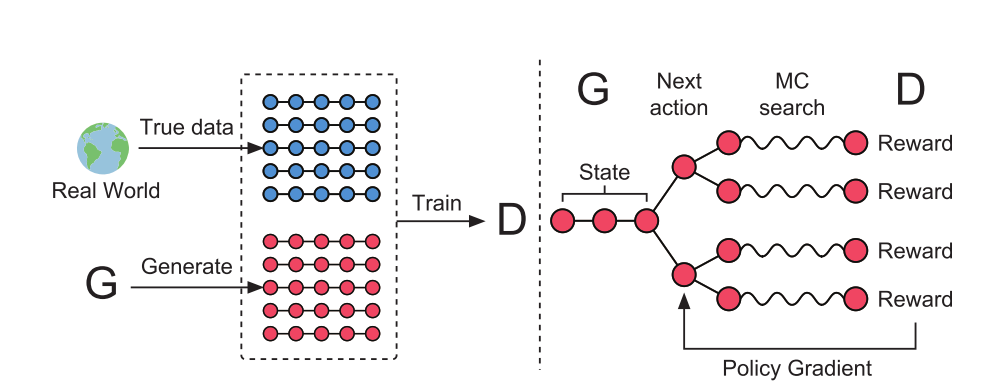
\includegraphics[width=20em]{figures/SeqGAN-general-structure.png}
		\end{figure}
		\vspace{-1em}
		\begin{itemize}
			\pause
			\item Left: $D$ is trained over the real data and the generated data by $G$.
			\pause
			\item Right: $G$ is trained by policy gradient where the final reward signal is provided by $D$ and is passed back to the intermediate action value via Monte Carlo search.
			\pause
			\item Ths discriminative mode $D_\phi$ is trained by providing positive examples from the real sequence data and negative examples from the synthetic sequences generated from the generative model $G_\theta$.
			\pause
			\item At the same time, the generative model $G_\theta$ is updated by employing a policy gradient and MC search on the basis of expected and reward received from the discriminative model $D_\phi$.
		\end{itemize}
	\end{frame}

	\section{Q\&A}
	
	%\part{Neural Dialogue Generation}
	%\subtitlepage{}{Adversarial Learning for Neural Dialogue Generation}{Jiwei Li, Will Monroe, Tianlin Shi, Alan Ritter and Dan Jurafsky\\arXiv: 1701.06547}
	%\begin{frame}{Introduction}
	%	\begin{itemize}
	%		\item Open domain dialogue generation aims at generating meaningful and coherent dialogue responses given input dialogue history.
	%		\item In this paper, authors discussed potential pitfalls of adversarial evaluations and necessary steps to avoid them and make evaluation reliable.
	%		\item This approach produces more interactive, interesting and non-repetitive responses than standard SEQ2SEQ.
	%	\end{itemize}
	%\end{frame}
\end{document}